% !TeX root = ./main.tex

\documentclass[10pt,b5paper,twoside,openright, english]{book}


\usepackage[utf8]{inputenc}


\title{Semesterprojekt}
\author{Jørn Bøni Hofstad}

\date{\today}


\usepackage{semester_project_packages}
\addbibresource{main.bib} % This is for biblatex to know what the bibliography file is


\begin{document}

\begin{titlepage}
    \begin{center}
        \vspace*{1cm}
        \Large
        \textbf{Representation of time-delay in state-space models of power electronic systems}
  
        \vspace{0.5cm}
        
        \normalsize
        \textbf{Jørn Bøni Hofstad}
        \vspace{1.5cm}
        
        Semester-project
        \vspace{1.8cm}

        Supervisor:\\
        Jon Are Wold Suul\\
        Associate professor\\
        Department of Engineering Cybernetics
  
        \vfill
  
  
        \vspace{0.8cm}
  
        
        Department of Engineering Cybernetics\\
        Norwegian University of Science and Technology \\
        Norway\\
        \today

        
\includegraphics[width=0.4\textwidth]{Figures/university.pdf}
  
    \end{center}
 \end{titlepage}

\frontmatter
\tableofcontents
% \newpage
\printglossary[type=\acronymtype,title={List of Acronyms}]{}
\printglossary[title={List of symbols}]{}
\chapter{Introduction}


\section{Abstract}
Normally, when handling time-delays, Padé-approximations are used to estimate the delay. Although they asymptotically give the same response as a time-delay, there are no guarantees for how they will act in reality when they are interconnected. Discretising the system into the z-domain provides exact solutions, but the space is quite distorted and very dependent on the sampling rate. Analysis in the z-domain tends to be difficult as a result. This project report proposes the usage of the w-transform with to give estimates that may provide a more accurate analysis of robustness, and who provide stronger guarantees for the quality of the estimate.

The way this will be done will be to give exact solutions for all continuous parts by assuming that all outputs from the controllers are zero-order hold. After that, the exact solutions will be used together with the control laws for the internal states in the controller, as well as a state, representing the delayed input. The resulting closed-loop system will then be transformed into the w-domain, where it can be analysed. When analyzing the sensitivity to modeling errors, the eigenvalues of the closed-loop matrix is differentiated with respect to a physical parameter. Which means stepping back through the transformation by using the chain-rule. The expression can not be differentiated exactly, so an estimate is given instead, as well as an upper bound on the magnitude of the error. 

\section{Sammendrag}
\todo[inline]{Legg inn et sammendrag som sier det samme som abstractet}
Når man jobber med tidsforsinkelser tar man som oftest i bruk padé-approksomasjoner. Selv om de asymptotisk gir samme respons som en tids-forsinkelse er det ingen garantier for hvordan de vil fungere i praksis om flere er koblet sammen i et lineært system. Det er mulig å ta i bruk diskretisering, siden det gir eksakte løsninger, men z-domenet er ganske forvrengt, og veldig avhengig av samplings-rate. På grunn av dette kan det være vanskelig å bruke z-domenet til stabilitetsanalyse. I dette prosjektet foreslås det å bruke w-transformasjonen i stabilitetsanalysen for å få estimater som forhåpentilgvis er mer presise, og som også kan gi sterkere garantier for kvaliteten av estimatet. 
\chapter{Preface}
\todo[inline]{Complete the preface}
This document is a semester-project report that was written during the autumn-semester of 2019 at the Norwegian University of Science and Technology (NTNU). The project was done under the supervision of associate professor Jon Are Wold Suul. Throughout the semester, he provided information about electrical three-phase circuits, the w-transform, certain characteristics of the w-transform and methods for tuning SISO-systems. All data-plots in the report were made using Python 3, and all simulations of the three-phase system were done with Matlab and Simulink. The figures that are not explicitly referred to as originating from somewhere else were made in Microsoft Visio. In this project, it is assumed that the reader has some basic knowledge of electrical circuits and three-phase power, as well as at least some understanding of linear algebra and linear dynamic systems. Finally, Morten Dinhoff Pedersen helped to highlight the problem with using the trapezoidal rule for estimation, and Harald Hanche-Olsen helped with mentioning a method for how to give an upper bound to a set of matrix-multiplications. 


\begin{center}
 \textbf{Jørn Bøni Hofstad}
 \today
\end{center}
\chapter{Introduction}


\section{Problem description} %#TODO See if this is a part is needed \todo[inline]{See if this is a part is needed}
Power electronic converters are increasingly utilized as the grid interface of generation systems and loads in ac power systems. The tuning of conventional cascaded control systems for such power electronic converters can have a significant impact on the stability and dynamic response of the converter as well as local power systems. Linearised state-space models are commonly utilized for assessing the small-signal stability and controller tuning of traditional power systems as well as for modern power systems with increasing share of power electronic converters. However, the time-delays in the control system implementation for power electronic converters have a significant influence on stability but cannot be easily represented in continuous time state-space models. Accurate stability analysis of power electronic converters with low sampling frequency can be based on discrete-time models, but such models of individual power electronic converters in the z-domain cannot be easily integrated with continuous-time state-space models (or s-domain models) of larger systems. Furthermore, many of the tools for eigenvalue-based analysis of small-signal dynamics, parametric sensitivity and interaction analysis by participation factors are not easily applicable in the z-domain. This project should evaluate how bilinear transformations can be utilized for an accurate representation of time delays in traditional state-space models of power electronic converters that will be suitable for integration in larger system models for eigenvalue-based analysis of small-signal dynamics.


\section{Motivation}

\todo[inline]{What is the motivation for considering the problems/questions that you approach in your work? Why is this an interesting problem? The motivation should instead describe why it is interesting from a societal point of view, and/or from a scientific point of view.

Remember to clearly cite what has been done earlier on the topic, to put your work in the correct context: In source(1) a control law is defined which..., while source(2) considers the particular case of... However, in these works... and in this work we will extend this by... / we will instead .... In "Reference to your own pre-project" a literature review was performed, showing that there is a need for ... Moreover, a preliminary controller was developed which ..., but has the drawback that... In this thesis, we will instead ... / we will further develop this control law by utilizing the control method XX... 

Figures are referred to as follows: In Fig.~1 you see an interesting curve. There is also a table in this sample report: Table~1.
}
%! Here starts my own part 
The issues concerning sampled systems and the problems that arise from the resulting time-delays is something that has been thoroughly explored \cite{Suul_paper_2,RegTek_boken}. Usually, analysis of sampled systems is either done in continuous time with an estimation of the delay \cite{RegTek_boken} or in the discrete-time-domain\cite{Suul_paper_2, Disc_paper}. Although Padé-approximations can give excellent estimates in \gls{SISO}-systems, it can be difficult to know all the consequences of using it in the \gls{MIMO} case. Whereas in the discrete-time domain, the tools that are normally used don't work anymore, since the stability region is within the unit circle instead of the left half-plane. This Project-report, we will propose a method for finding pessimistic estimates for the stability margins of mixed continuous-discrete systems with high requirements for robustness. 

\section{Literature review}
All required details to model a three-phase system were given in \cite{eth_paper, Suul_paper_1,Suul_paper_2,Suul_electro_presentation_1}. The mathematical background for Jordan-blocks and eigenvalues was given in \cite{LinSys_boken}. Background for analysis of robustness, as well as the w-transform, came from \cite{RegTek_boken}. Information about matrix-norms and operator norms was found in \cite{Triangle_inequality_source}. Whereas methods for differentiating matrices came from \cite{Matrix_differentiation_source}
\noindent
It is quite possible that there already exist methods in the literature that are similar to what has been proposed in this project-report, but as of when \todo[inline]{Hvordan bør dette formuleres} the methods were developed, no such methods were known, beyond the fact that several of the results seem to come rather naturally from the already known tools that were known and that were needed for the project. 

%#TODO Left off here (Bør denne være her)
\section{Assumptions}
In order to make the analysis somewhat feasible to perform, it was assumed that all components in the grid were ideal. Additionally, it was also assumed that the sampling-rate was constant and that there were no other sampled systems affecting the same continuous subsystems. Most importantly, it was assumed that the system was sufficiently linear for small-signal analysis to be applicative. Finally, it is also assumed that all matrices $\Vec{A}$ are dependant on some unspecified parameter $\rho$ that acts as a placeholder for any of the physical parameters. 
\noindent 
Unless stated otherwise, all figures are made by me. All mathematical proofs were not credited to somebody else were made as a part of this project, without the knowledge of how the original proofs were made, or if they existed. \todo[inline]{Dette betyr at jeg må gå over alle bevisene og refferer de til kilder. Dette kan bli problematisk}%#TODO Formulering med tid, og riktig person-form, og muligens hvordan dette egentlig skal formuleres. 


\todo[inline]{Include this section if it is necessary to state some assumptions that you have made to restrict the scope of the thesis.}

\section{Related work}
The idea of using the w-transform when analyzing discrete-time systems has already been proposed in \cite{Suul_paper_2}. But, there, the main focus was on- tuning, instead of stability analysis.
\noindent
The entire concept of transforming three-phase systems so that they can be perceived as time-invariant problems seems to be thoroughly explored\cite{Suul_paper_1,Suul_paper_2,eth_paper}. The same goes for Phase-locked loop \cite{Suul_paper_1, eth_paper} and the derivatives of matrices with respect to specific parameters \cite{Matrix_differentiation_source}. Everything about matrix-norms is a part of classical linear algebra and has probably not been anywhere near relevant or new in the last hundred years \todo[inline]{Hvor fritt bør jeg formulere meg}. 


\section{Contributions}

The main contribution of this project is joining all the required steps needed to get a decent transformation of a sampled, continuous \gls{MIMO}-system with a discrete controller into the w-domain. More importantly, was the development of a non-general method to give an upper bound to the derivative of the system-matrix in the w-domain with respect to physical parameters in the continuous time-domain. The results of this project are limited to systems where, if the continuous-time system-matrix has any eigenvalues equal to 0, the eigenvectors of such a subspace must be unaffected by all uncertain parameters. 
\noindent 
The appendix also contains a method for finding exact responses of linear time-invariant systems that work for inputs that are described by arbitrary, finite polynomials. Although no mention of the technique was found elsewhere, it is highly unlikely that this has not already been discovered. Simply because of how intuitively a general proof comes from proving the exact solution of a step-response by using a Taylor-series.

Finally, in order to model the controller connected to the continuous grid, a model had to be provided, where everything was translated into the dq-reference frame and where the parameters of the controller were separated from the dynamics of the continuous system. 
\noindent
\todo[inline]{Bør jeg legge til delen med vilkårlige polnom, og delen med den oppsatte modellen. Det er høyst sannsynlig at den ikke er unik }
\todo[inline]{Hva man selv har utviklet}



\section{Outline}
The report is organized as follows: \todo[inline]{Kanskje ha en bedre formulering på dette}
\begin{itemize}
 \item \Cref{chp:Modeling_the_grid}: All the necessary background is given for modeling a three-phase grid as a time-invariant system. There is also information on how to write the system on per unit-form, which allows for making a generalized grid, that can be scaled to arbitrary frequencies and operational values later. 
 \item \Cref{chp:VSC}: Describes a \gls{VSC}, both in structure, and what the different components do. As a part of this, the \gls{PLL} is described. In addition, en example of a current-controller is given, although, it is possible to have several different kinds of architecture, depending on the control objective, so a current-controller is not always the thing that is used. 
 \item \Cref{chp:z_transform}: How to perform the z-transformation, both by the trapezoidal rule from the z-domain and with an exact solution from the continuous-time domain. 
 \item \Cref{chp:w_transformation}: Explains the w-transformation, as well as some intuitive explanations on why analysis in the w-domain might be preferable to analysis in the z-domain. 
 \item \Cref{chp:linearize_the_system}: How to linearize the nonlinear equations that describe the controller and the grid, while also including the linearized control laws in the z-domain. Finally, the chapter sets up the entire closed-loop system on matrix-form 
 \item \Cref{chp:new_findings}: Explains the new contributions from this project and most of the algorithm for performing stability-analysis if the system-matrix is invertible. 
 \item \Cref{chp:conclusion}: Conclusion, as well as potential further work
 \item \Cref{chp:discussion}: Goes over some of the consequences of the findings that were made. It also covers part of what kinds of problems that can be solved with the methods derived in this project. 
 \item \Cref{chp:appendix}: Mostly contains some of the proofs and explanations that were a bit too long or involved to be in the main text. But they are still essential for the results. The response for polynomial inputs, as well as what to do if the system-matrix is non-invertible or defective is here. Finally, an explanation of a PWM is delegated to the appendix, since is expected to already be known by most readers. 
 
\end{itemize}
% \todo[inline]{The report is organized as follows. In Chapter~1 a mathematical model is developed to describe the system... In Chapter}


\mainmatter
\chapter{Modelling the grid}
\label{chp:Modeling_the_grid}
\section{Voltage-converters in grids}
\label{sec:VSC}


\begin{figure}[ht!]
 \centering
 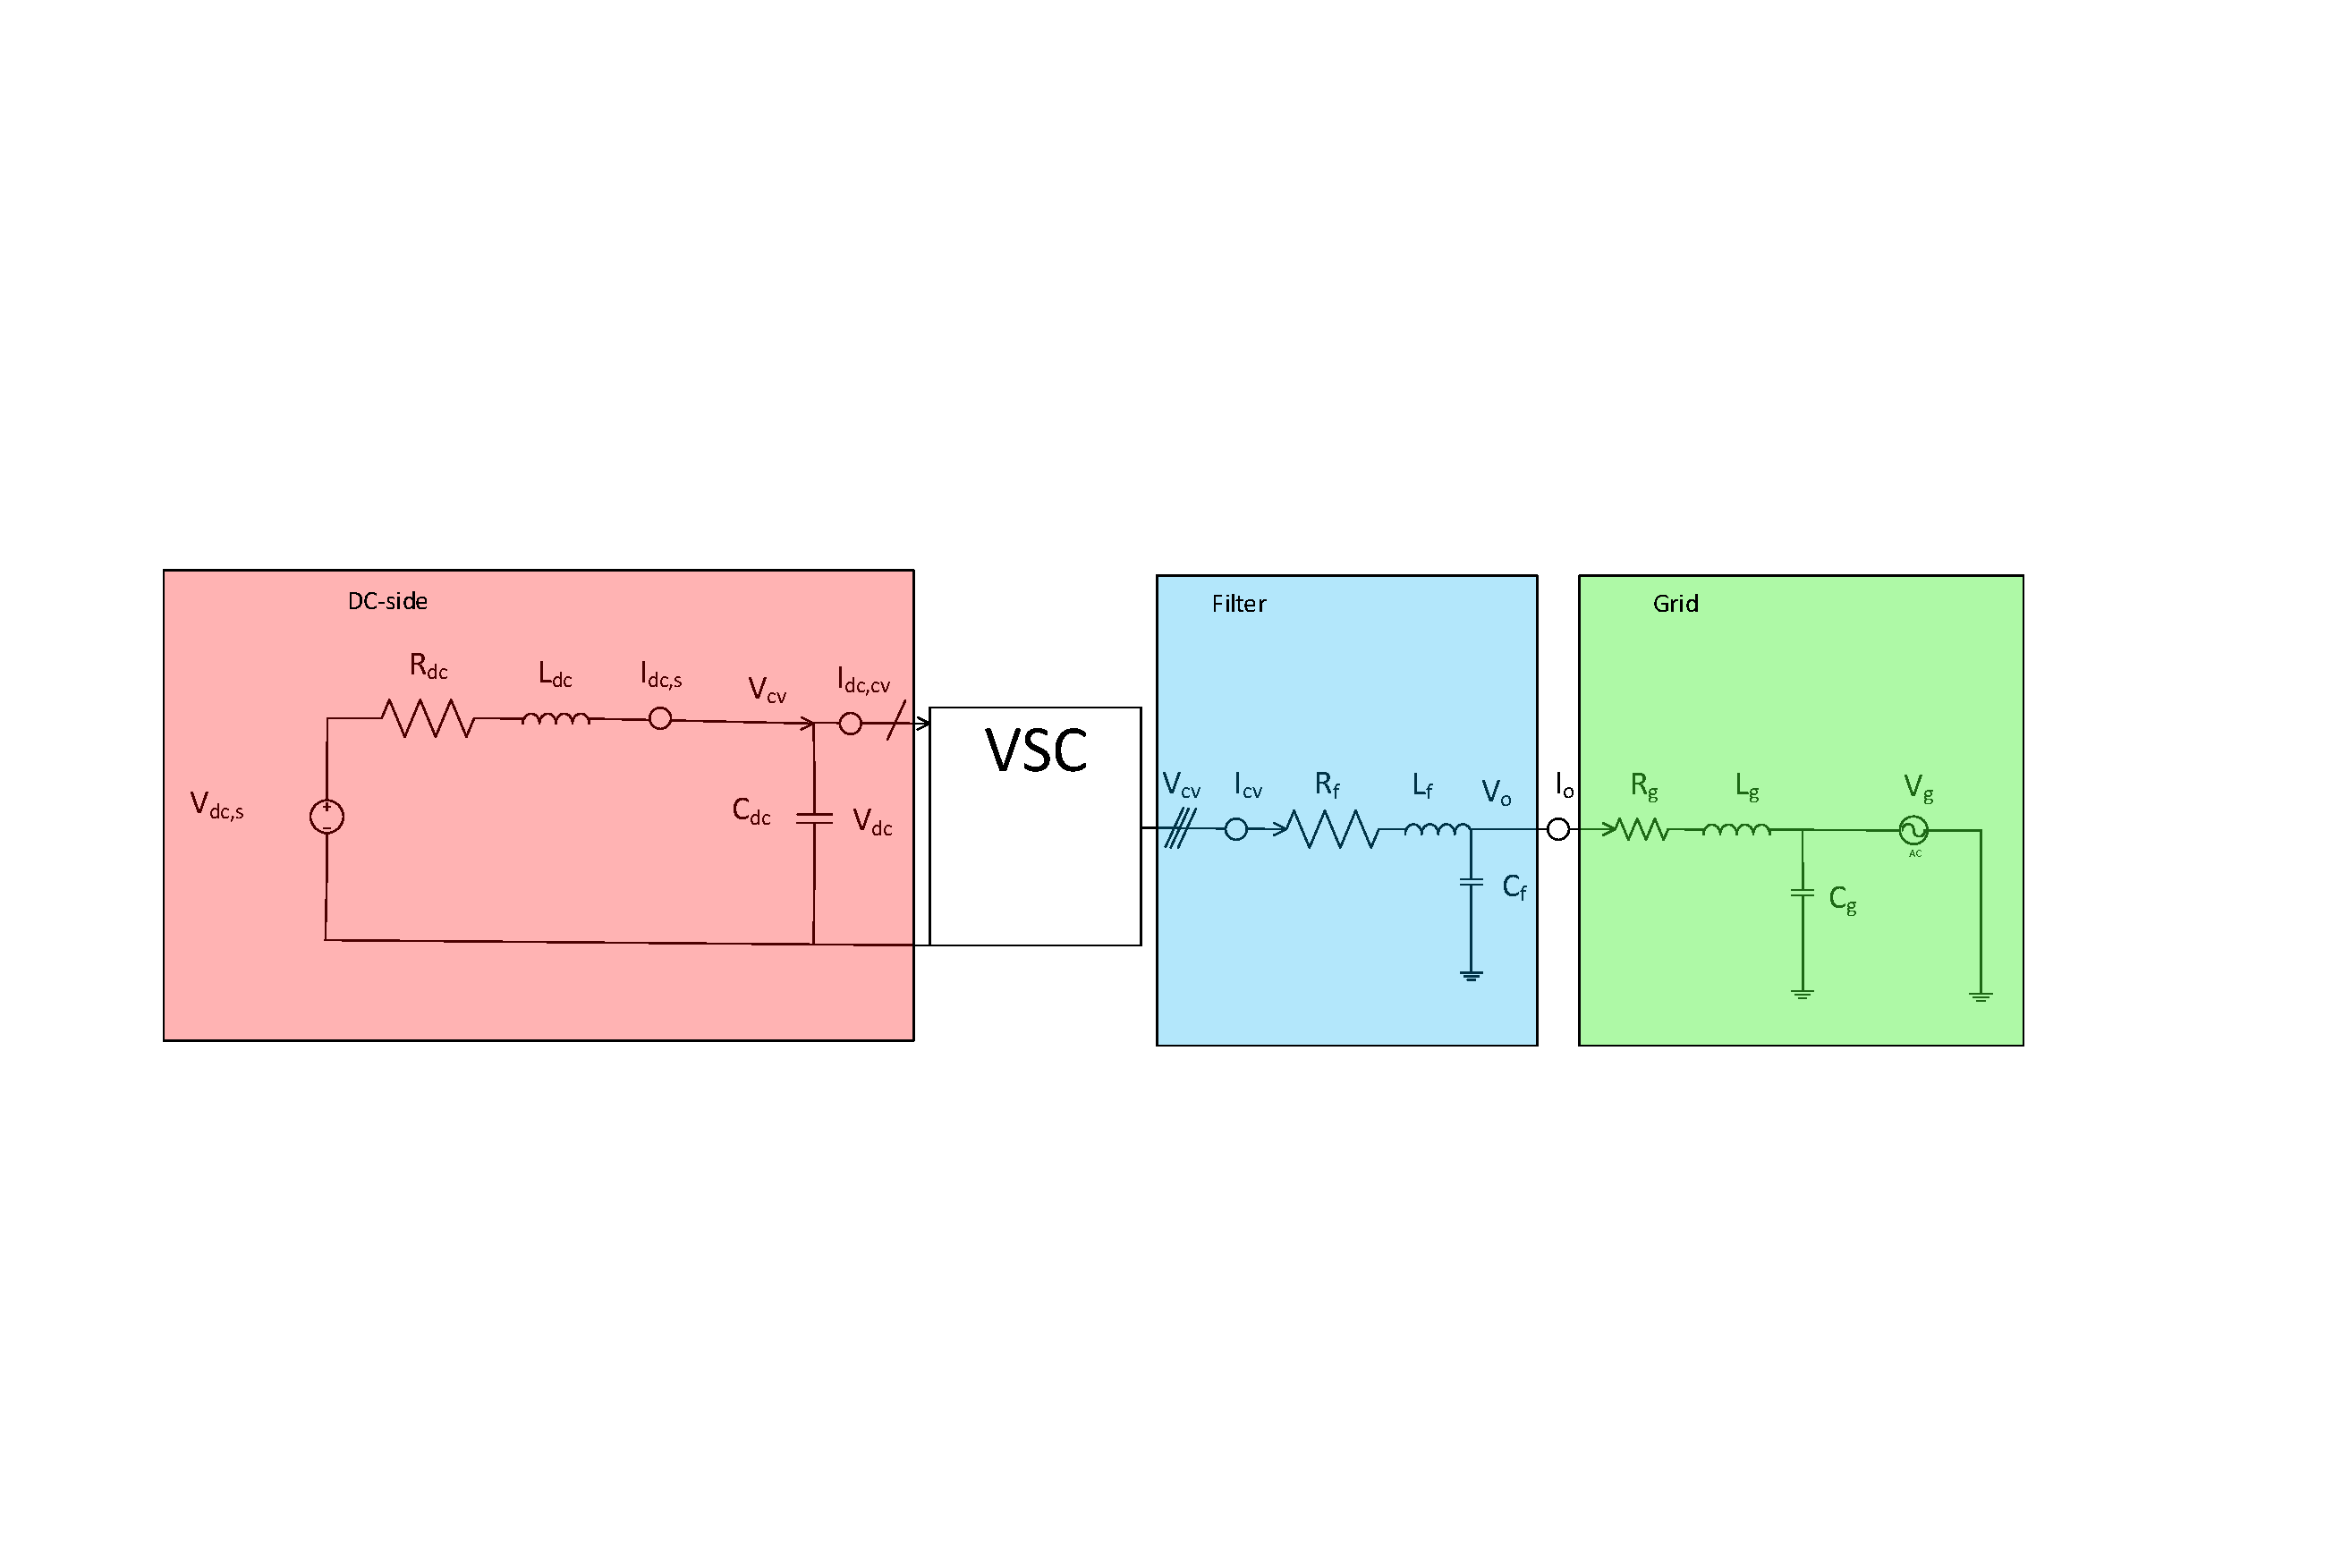
\includegraphics[width=\textwidth,height=\textheight,keepaspectratio]{Figures/Sectioned_simplest_transformer.pdf}
 \caption{The circuit with the VSC as a black box. The components are divided into sections for clarity}
 \label{fig:simplest_system}
\end{figure}


In order to connect a DC-voltage source to an AC power-grid, some kind of transformation is needed. Usually, this is done with a \gls{VSC}, as sin in \cref{fig:simplest_system}. We will represent the internal impedance by the components R\gls{_dc}, L\gls{_dc} and C\gls{_dc} on the dc-side side of the \gls{VSC}. In order to create a smooth current and voltage from the voltage \gls{V_cv}, and the current \gls{I_cv}, a first-order continuous filter is made. The filter is made up of R\gls{_f},L\gls{_f} and C\gls{_f}. For simplicity, the output of the \gls{PWM} is assumed to be a piecewise constant signal, even though it, in reality, is a duty-cycle. The grid can be modeled in a lot of different ways, depending on if there are other components, or if it is a strong grid. The simplest possible model is with a strong grid, which means the voltage of the grid is an AC-voltage that does not change depending on the current given or taken to the grid. 

As seen in \cite{Suul_paper_1}, the internal impedance and the line-impedance on the DC-side can be modeled as a pi-equivalent ( an inductor and a resistor in series, followed by a capacitor in parallel). Also, any capacitance at the terminal is simply added as a part of the inductor. The line-impedances along in the AC-grid can also be lumped together into a pi-equivalent, just like in \cite{Suul_paper_1}
\noindent
%#TODO Legg finn ut hvor jeg skal skrive om VSC-en
If a \gls{PWM} is supposed to be able to follow the voltage from somewhere else, it needs to know the phase and frequency of the rest of the grid. Since none of these are known exactly, some kind of measurement is needed to provide them instead. This is where the \gls{PLL} comes in. The \gls{PLL} is a part of the \gls{VSC}. It takes the measured voltage at the output of the filter and is give an output that converges towards the actual angle and angular velocity of the grid. The \gls{PLL} is discussed further in \cref{sec:PLL}


\begin{figure}[ht!]
 \centering
 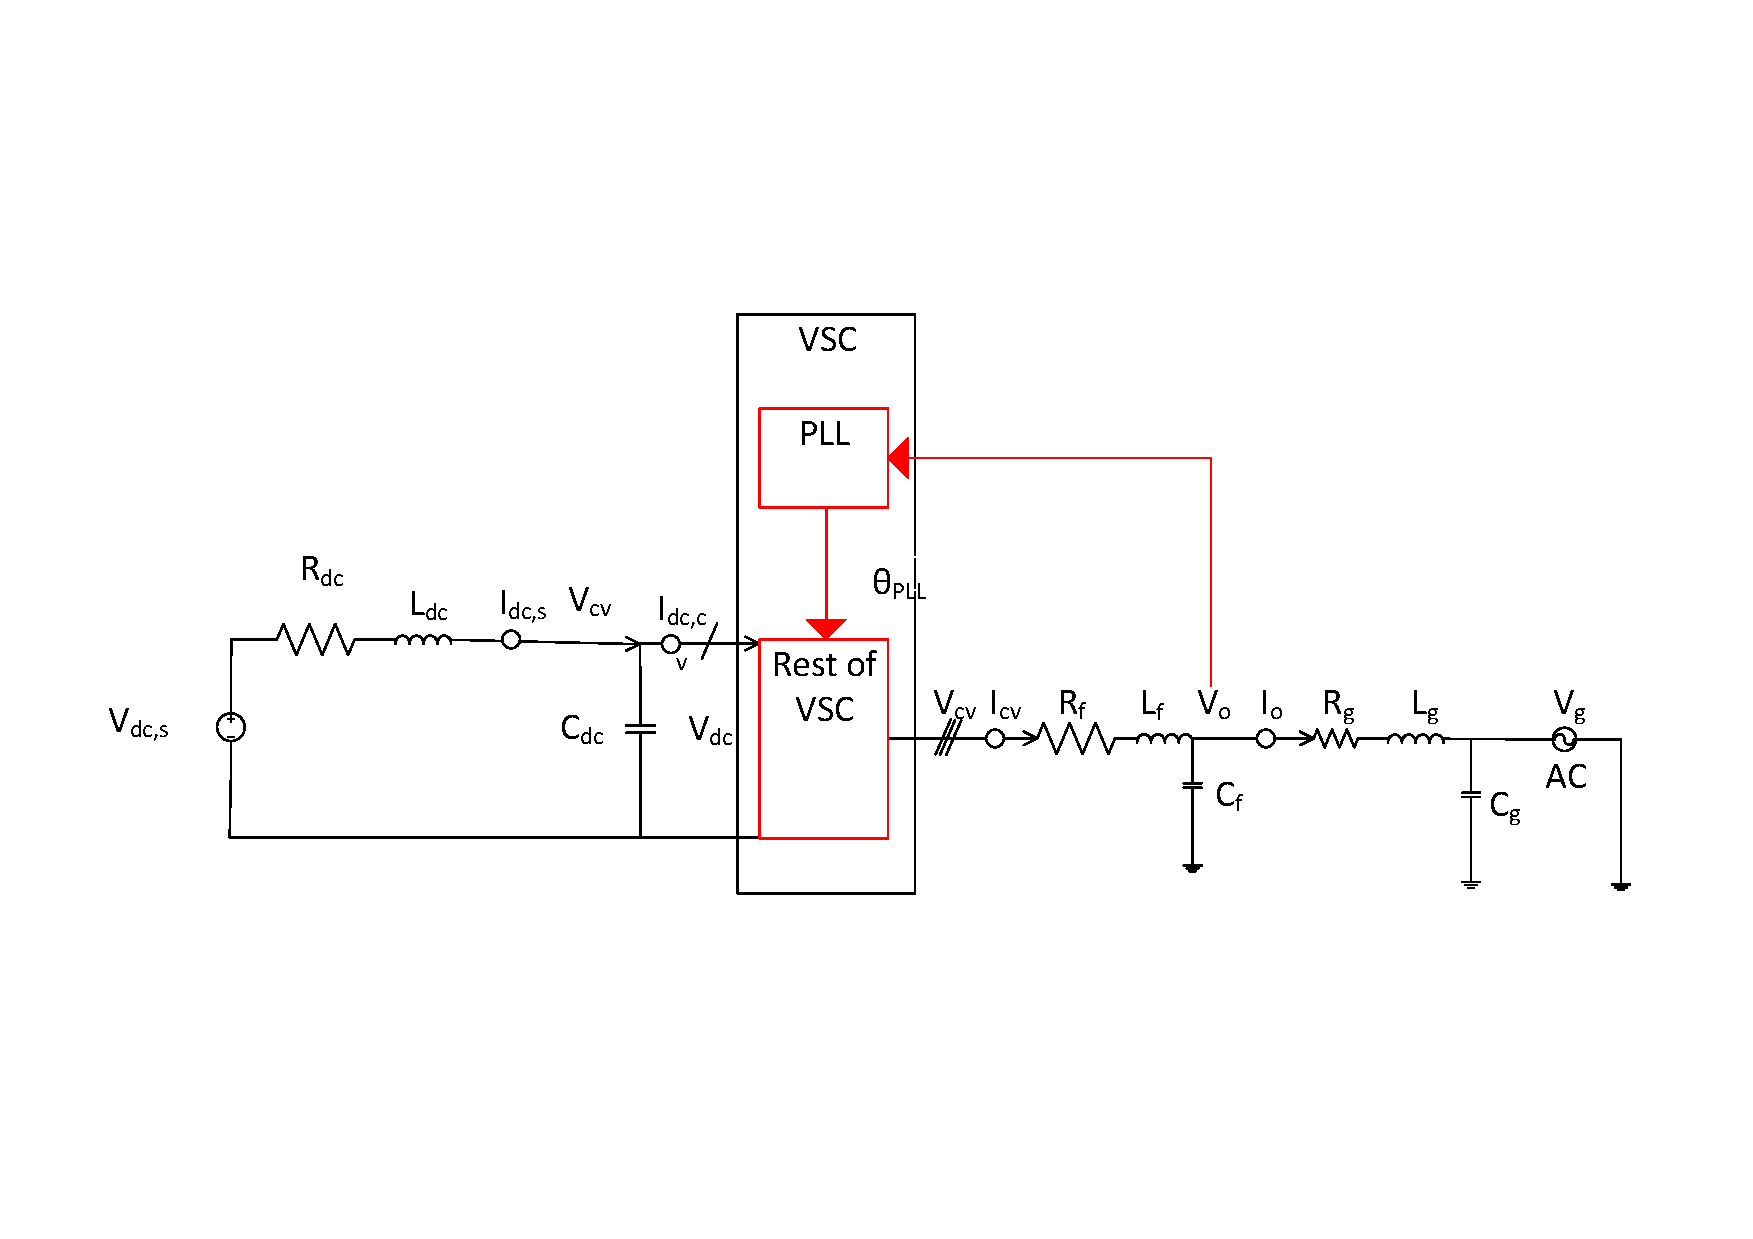
\includegraphics[width=\textwidth,height=\textheight,keepaspectratio]{Figures/Transformer_with_PLL.pdf} %#TODO Make a better figure that adds the PLL to the VSC
 \caption{The \gls{PLL} is a part of the \gls{VSC} that gives an estimate of the phase, which is reeded for the rest of the \gls{PLL} to function. It will be discussed properly in \Cref{sec:PLL}}
 \label{fig:curcuit_with_pll}
\end{figure}

A normal PI-controller will not be able to follow an oscillating reference that has an unknown frequency without suffering from stationary deviations. The solution for this is to use a rotating reference frame. 


\section{The Park transformation}

A proper explanation of the dqz- transformation is in \cref{sec:rotating_reference_frame}

The dqz-transformation can be seen as a projection from the normal reference-frame, abc, to a rotating reference-frame, dq. An alternating current that has the same angular velocity as the dq-reference frame will be perceived as a complex, stationary DC-current instead in the dq-frame. For a balanced system, the transformation is given by the matrix

\begin{equation}
 K_{CP} = 
 \frac{2}{3}\begin{bmatrix}
 \cos{\left(\theta\right)}
 & \cos{\left(\theta - \frac{2\pi}{3}\right)}
 & \cos{\left(\theta + \frac{2\pi}{3}\right)} \\
 -\sin{\left(\theta\right)}
 & -\sin{\left(\theta - \frac{2\pi}{3}\right)}
 & -\sin{\left(\theta + \frac{2\pi}{3}\right)} 
\end{bmatrix}
\end{equation}{}

The third state is a scaled sum of all phases, but since all phases are supposed to add up to 0 together in a balanced system, they are ignored here. 

\noindent
The transformation makes it possible to view the control problem as time-invariant. This is because the reference signal from the grid-voltage will no longer have to be viewed as three oscillating sine-waves, but instead as two signals that will remain constant as long as the grid-voltages continue to oscillate with the same amplitude and frequency. This is especially useful since linear regulators have no way to follow an arbitrary single frequency without phase-delay.

\section{Per unit systems}
Normally, an electrical system is designed with regard to some specific physical parameters. This means that using the same design for systems with different characteristics requires some thought when scaling all the parameters. 
Per-unit systems help to solve this by defining nominal values (The normal values of both components and states during "Normal operation"), and then designing the circuit with values that are expressed as multiples of the base-values instead. This makes it easier to use the same design for several different scenarios. It also makes it easier to see if observed values are abnormal or not, since everything is based around 1. Basis values for a per-unit system are always followed by a subscript b (like V\gls{_b}). A value that is given in per unit will always be written as a lowercase letter. Physical values, except for angular velocity $\omega$ are always written in upper-case. 


\begin{equation}
 v_g = \frac{V_g}{V_b}
\end{equation}{}

In order to get a per-unit system, some base values have to be defined. These are usually $P_b$, $\omega_b$ and $V_b$. Take note that $\omega_b$ breaks the convention since all angular velocities are all given by a small $\omega$, regardless if they are per unit or not. The grid frequency \gls{omega_g}, estimated grid frequency $\omega_{PLL}$ and basis frequency $\omega_b$ are all written in lower-case, even though only the first two are in per unit. We do this because large $\Omega$ usually refers to a resistance of some sort. As a result: 
\begin{equation}
 \gls{omega_g} = \frac{\omega_{g, physical}}{\omega_{b}} 
\end{equation}
\section{Circuit equations}
As seen in \cite{Suul_paper_1}, the internal impedance and the line-impedance on the DC-side can be modeled as a pi-equivalent (An inductor and a resistor in series, followed by a capacitor in parallel). Also, any capacitance at the terminal on the DC-side described within the capacitance in the pi-equivalent. The filter is a simple RLC-filter, just like what can be seen in \cref{fig:simplest_system}.

In order to get the circuit equations for the dq-reference frame, some assumptions and observations have to be made. 
Firstly, the $\alpha\beta$-frame is just a constant linear combination of the abc-frame. This means that, due to linearity, the differentiating variables in the $\alpha\beta$-frame will act exactly like the ones in the $abc$-frame. 
Also, anything in the dq-frame can be represented as $v_{dq} = e^{-j\theta_{PLL}} v_{\alpha\beta}$. As long as the angular velocity remains constant, it can be written as $v_{dq} = e^{-j\left(\omega_{PLL} t + \phi \right)} v_{\alpha\beta}$. This means that 
\begin{equation}
 \frac{d \left( i_{dq} \cdot e^{\omega_b t}\right) }{dt} = e^{\omega_b t} \left( \omega_b i_{dq} + \frac{d i_{dq}}{dt} \right) 
\end{equation}
As a result, differentiation in the dq-frame acts differently than in the $\alpha\beta$-frame, but can still be done. 
Finally, the fact that $I_b R_b = I_b \omega_b L_b$ in the dq-frame is also used to get the normal circuit-equations on per unit form. As a result the circuit equations can be written as in \cite{Suul_paper_1}: 


\begin{align}
 \frac{d \Vec{i\gls{_cv}}}{dt} &= \frac{\omega\gls{_b}}{l\gls{_f}}\Vec{v_{cv}} - \frac{\omega_b}{l_f}\Vec{v}\gls{_o} - \left( \frac{r_{l_f}\omega_b}{l_f} + j\gls{omega_g}\omega_b \right) \Vec{i_{cv}}\\
 \frac{d \Vec{v\gls{_o}}}{dt} &= \frac{\omega\gls{_b}}{c\gls{_f}}\Vec{i_{cv}} - \frac{\omega_b}{c_f}\Vec{i}\gls{_o} - j\gls{omega_g}\omega_b \Vec{v_{o}}\\
 \frac{d \Vec{i\gls{_o}}}{dt} &= \frac{\omega\gls{_b}}{l\gls{_g}}\Vec{v_{o}} - \frac{\omega_b}{l_g}\Vec{v}\gls{_g} - \left( \frac{r_{g}\omega_b}{l_g} + j\omega_g\omega_b \right) \Vec{i_{o}}\\
\end{align}{}



And on the DC-side, they are:
\begin{align}
 \frac{d v\gls{_dc}}{dt} &= \frac{\omega_b}{c_{dc}}\gls{i_dc,s} - \frac{\omega_b}{c_{dc}}i\gls{_dc}\\
 \frac{d \gls{i_dc,s}}{dt} &= \frac{\omega_b}{l_{dc}}\gls{v_dc,s} - \frac{\omega_b}{l_{dc}}v\gls{_dc}
\end{align}{}
\chapter{Voltage-source converter}
\label{chp:VSC}

Finally, we can open the magical box that we previously just said converted the voltage from DC to AC. From what we see right away in \cref{fig:internals_of_VSC}, we see that the \gls{VSC} contains a \gls{PLL}, a \gls{PWM}, a controller, as two blocks performing the Park and the inverse Park transform. From what we have seen up until now, the \gls{VSC} can affect the continuous circuit through three inputs $i_{dc}$, $v_{cv,d}$ and $v_{cv,q}$. Intuitively power can not come from nowhere, so there exists one constraint as well. The resulting system has two degrees of freedom. If the controller has two degrees of freedom, it is in theory possible to make it follow two control objectives. 

\begin{figure}[ht]
 \centering
 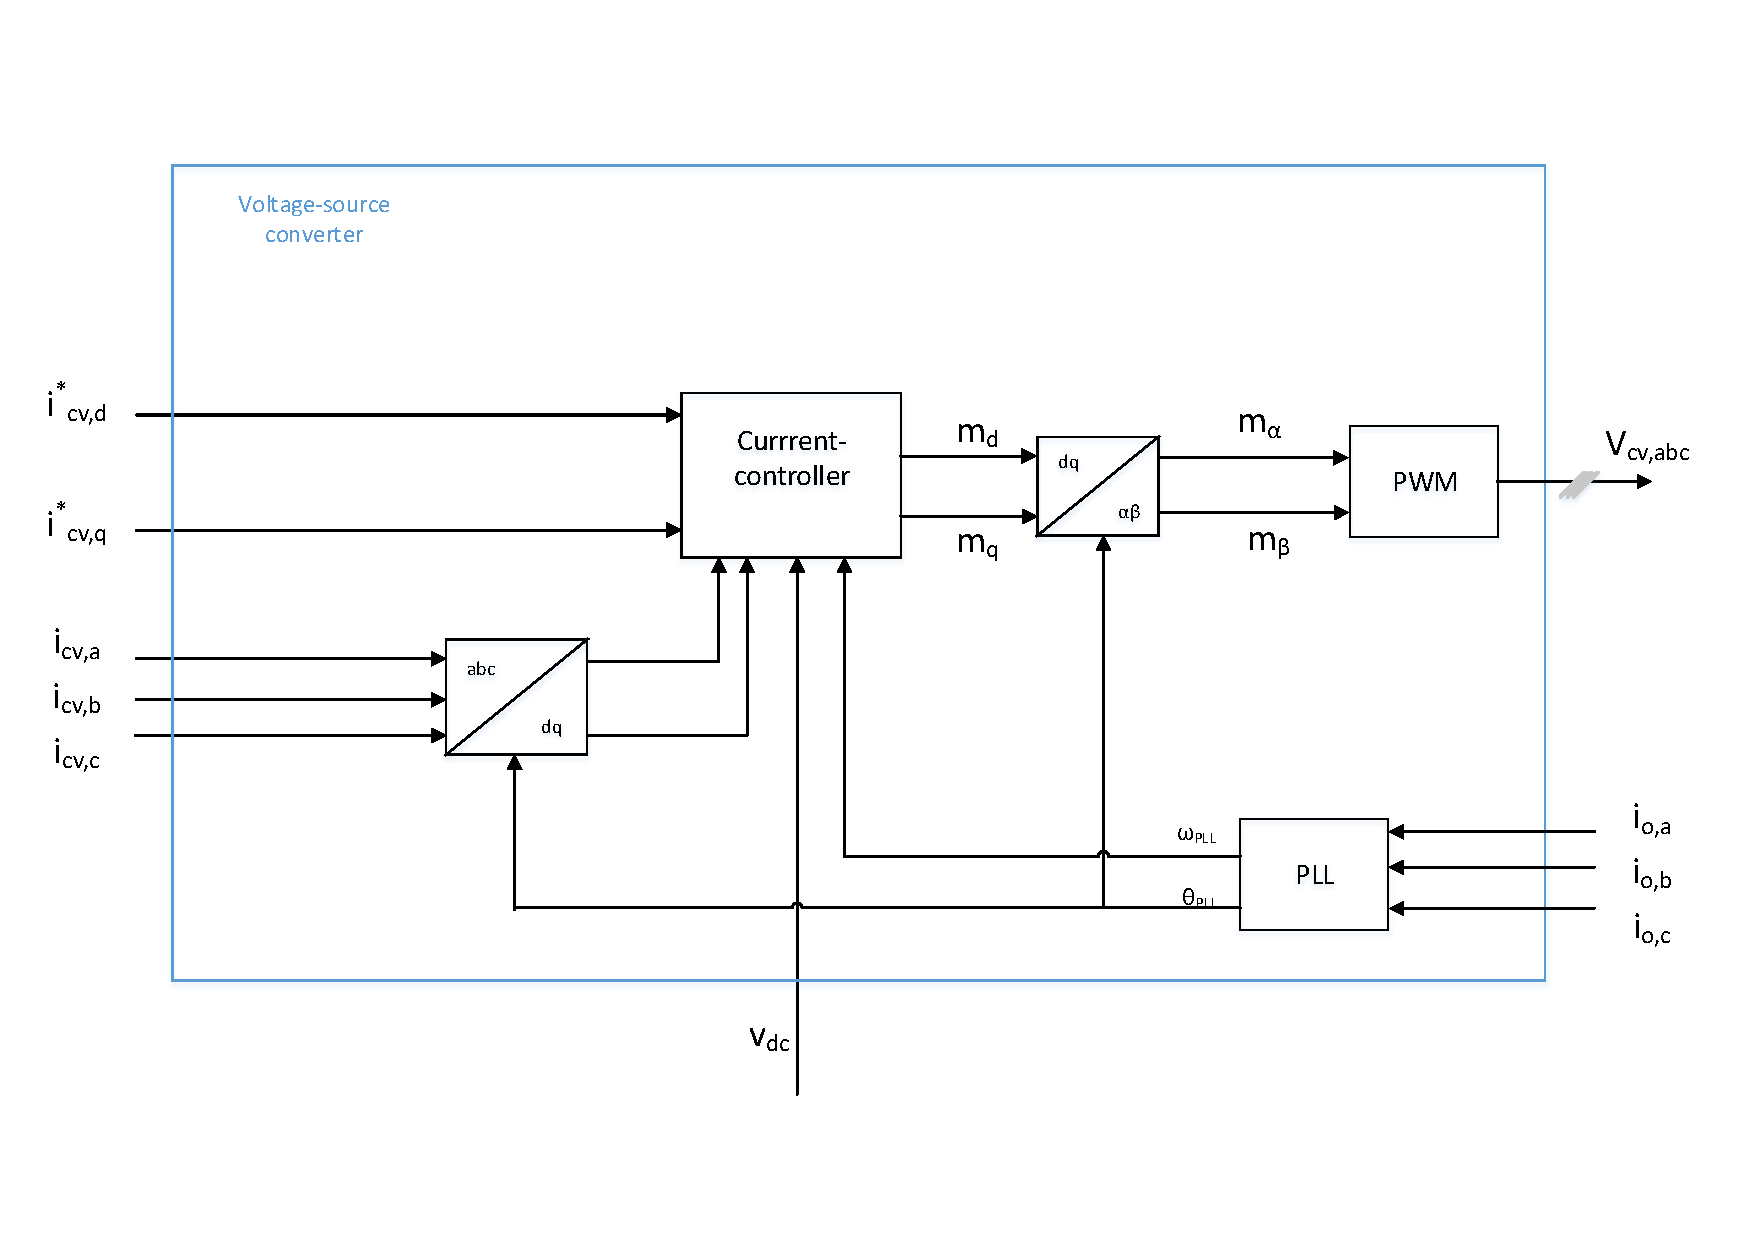
\includegraphics[width=\textwidth,height=\textheight,keepaspectratio]{Figures/Internals_of_the_converter.pdf}
 \caption{Voltage source converter (Inspired by \cite{Suul_electro_presentation_1})}
 \label{fig:internals_of_VSC}
\end{figure}{}
% \todo[inline]{Legg til nødvendig figur her}

As mentioned before, the \gls{VSC} contains a \gls{PWM}. A \gls{PWM} is described in more detail in \cref{sec:PWM}. But the short version of it is that it is able to give something that can almost follow a voltage reference by switching quickly between two voltages, which will give a smooth signal if it is passed through an RLC-filter. But the fact that the \gls{PWM} has to work on periodic cycles means that it has to be sampled. The time-delay in the system comes from the sampling that the \gls{PWM} has to do, as well as the sampling that is done to get the voltage and current measurements. 

\section{Phase Locked Loop (PLL)}
\label{sec:PLL}
In a grid, it is possible that the phase and frequency are not the same as what was first assumed when the system was designed. In order to remedy this, an estimate that tries to follow the actual phase of the grid has to be given instead. In order to do this, a PLL is used, which has a somewhat similar structure to a PI-controller, as seen in \cref{fig:PLL_fig}. The purpose of this controller is to reduce the perceived reactive voltage when using the estimated angle in order to transform the system from the $abc$ to the $dq$-frame. $atan2$ is a very non-linear mapping, so it makes more sense to filter both d and q before they are transformed into an angle by $atan2$. 

\begin{figure}
 \centering
 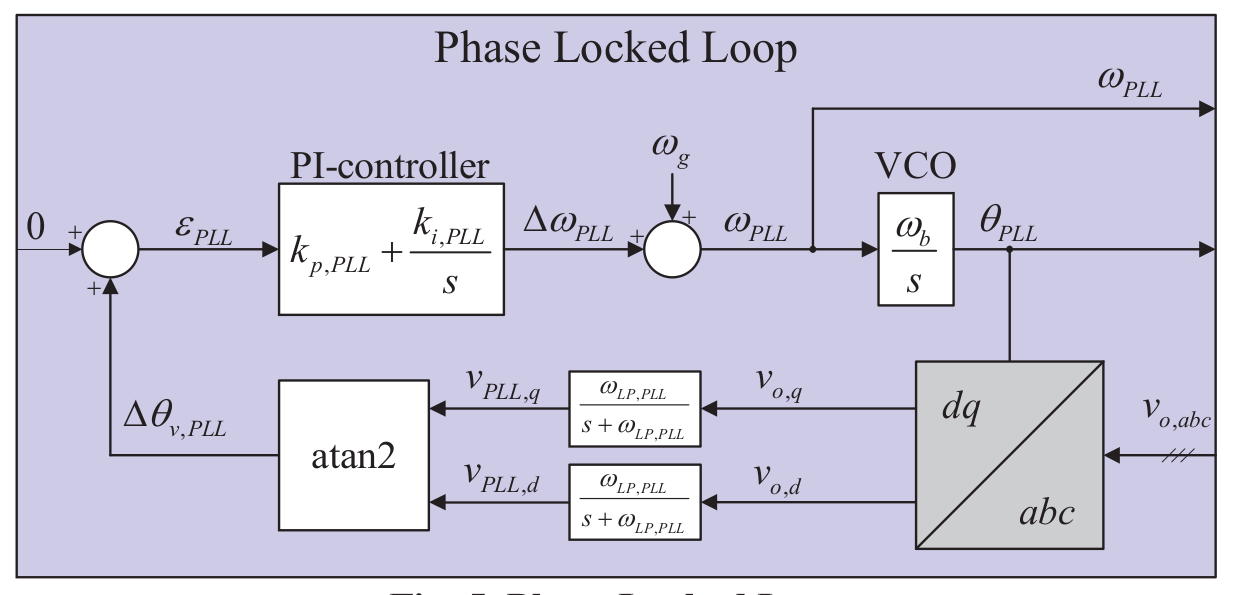
\includegraphics[width=\textwidth,height=\textheight,keepaspectratio]{Figures/PLL.png}
 \caption{Phase Locked Loop (\gls{PLL}), taken from \cite{Suul_paper_1,Suul_electro_presentation_1}}
 \label{fig:PLL_fig}
\end{figure}{}
 
Also worth noting is the term $\omega_g$, which is a result of fact that the controller is based on linearization around the expected operating frequency $\omega_g$. 

One final point to take special note of is the fact that the regulator uses the estimate $\omega_{PLL}$ for some feed-forward terms. Therefore, it is quite possible that the system may experience nonlinear characteristics as a result of the PLL. 

\section{Current-controller}

It is possible to have several different kinds of regulators, depending on what is needed. It is possible to regulate the active power on the AC-side, or the ammount of current drawn on the DC-side. Usually, these are controlled by giving some kind of reference to a current controller. But in our case, the controller will simply be a current-controller with nothing more. Since the PWM only is able to take in signals saying how long it should stay at the high or low voltage, the output AC voltage will be proportional to the input DC voltage. Because of this, it can often be good to get the modulation index by dividing the desired voltage by the measured DC voltage. 
\noindent
\begin{figure}[ht]
 \centering
 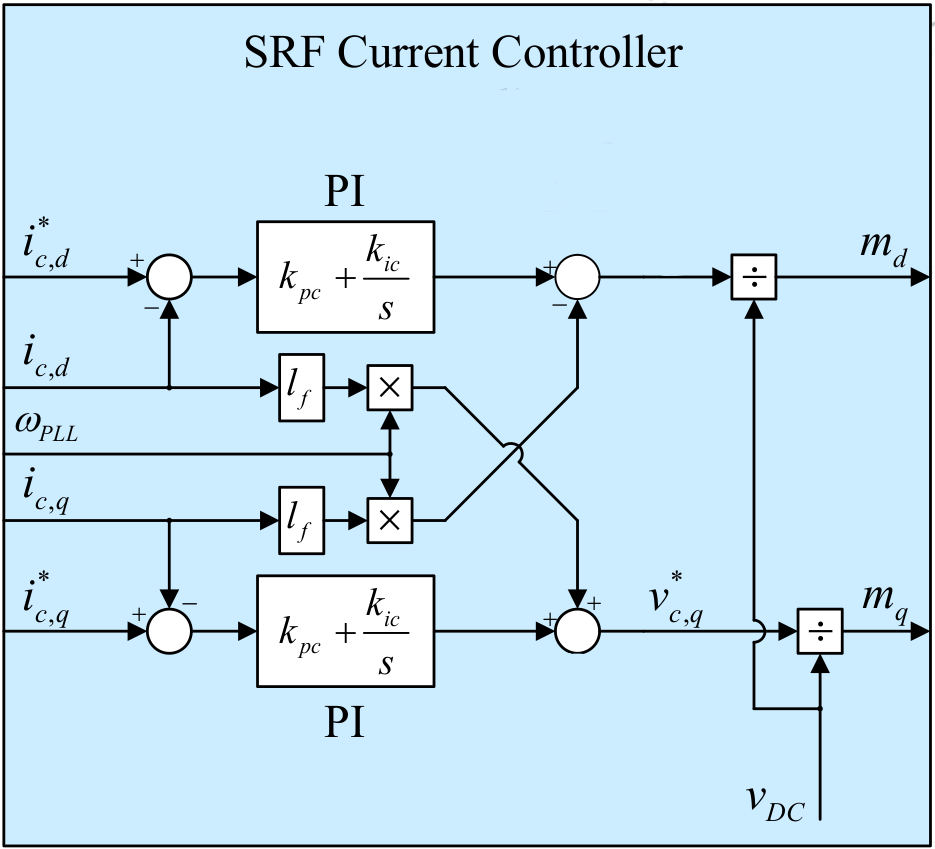
\includegraphics[width=\textwidth,height=\textheight,keepaspectratio]{Figures/stolen_controller_edit.png}
 \caption{Voltage source converter (Taken from \cite{Suul_electro_presentation_1,Suul_paper_1}, edited to reflect the equations used in this project)}
 \label{fig:decoupled_controller}
\end{figure}{}
When looking at the equations for the current in the controller, one term causes a lot of trouble. That term is $j\omega\gls{_g}\omega\gls{_b}\Vec{i_{cv}}$,since it couples the current in the d and q axis. This means that the d- and the q-current become them dependant on each other. In order to mitigate these problems, the decoupling terms $j l_f\omega_{PLL}$ are added. By adding the decoupling terms, the resulting matrix should become 
\begin{align}
 \frac{d \Vec{i\gls{_cv}}}{dt} &= \frac{\omega\gls{_b}}{l\gls{_f}}\Vec{v_{cv,PI}} + j\frac{\omega\gls{_b}}{l\gls{_f}}( l_f \omega_{PLL} ) - \frac{\omega_b}{l_f}\Vec{v}\gls{_o} - \left( \frac{r_{l_f}\omega_b}{l_f} + j\gls{omega_g}\omega_b \right) \Vec{i_{cv}}\\
\end{align}{}
So, if $\omega_{PLL} = \omega_g$ then, the terms will cancel, and the d and q-current will be decoupled. In theory, there are no guarantees that this will work perfectly, but in practice, it usually works quite well \cite{Suul_electro_presentation_1}
The remaining terms, which are represented by $\Vec{v_{cv,PI}}$ can be used by a PI-controller. The controllers can usually be tuned independently of each other. These can usually be tuned by Modulus optimum or symetrical optimum \cite{Suul_electro_presentation_1,Suul_paper_2}. In this case, the deviiation from a reference, for both active and reactive current is given as inputs to the controller. But, usually, if something else has to be controlled, a slower controller is normally used in order to give a reference to the current controller. 

\todo[inline]{Bør jeg legge til noe mer her? (Hvordan man tuner kontrollerne) }


\chapter{The z-transform}
Since our regulator is bound to be controlled by a micro-controller, part of the system is going to be sampled, and thus, it will act as a discrete system. Therefore, some of the tools for analyzing discrete-time systems are needed. 
\label{chp:z_transform}
\section{Characteristics of the z-transform}

The z-transform works similarly to the Laplace-transform, mapping a sequence $x(k T_s)$ to the z-domain, giving $x(z)$. If the values of $x$ only depend on the previous values, the system is causal, and we can use the one-sided z-transform to represent it. 

\begin{equation}
 x(z) = Z\{ x(k T_s) \} = \sum_{k=0}^\infty x(k T_s) z^{-k}
\end{equation}{}

The z-transform is notable, because it is a one-to-one transformation, meaning anything that can be transformed into the z-domain can also be inverse transformed back into the discrete time-domain. This is done by the inverse z-transformation. 
\begin{equation}
 \{x(k T_s)\} = Z^{-1}\{ x(z) \} = \frac{1}{2 \pi j} \int_C z^{k-1} x(z) dz
\end{equation}{}

Where C is a closed path around all poles in the z-transform. \todo[inline]{Gjøre denne delen mer presis}
Finally, when looking at the z-transform, it can be observed that

\begin{align}
 x(z) = Z\{ x((k+1) T_s) \} &= \sum_{k=0}^\infty x((k+1) T_s) z^{-k}\\
 &= (z\sum_{k=0}^\infty x(k T_s) z^{-k}) -x(0)
\end{align}
Which means that the factor $z^{-1}$ works as a time-delay operator for one time-step. 

\section{The effects of sampling}
When sampling a system, it is also worth noting that the sampling will introduce harmonics. 
Put simply, if you sample with a frequency of $T_s$
\begin{equation}
sin(\omega t) = sin\left((\omega + \frac{2\pi}{T_s })t\right) \forall t = n T_s : n \in \{...-1, 0,1,2, ...\}
\end{equation}{}
 As a result, the two sine-waves will be observed as the exact same signal. This phenomenon is known as aliasing and can occur for any signal that has a frequency that is faster than half the sampling frequency. This is known as the Nyquist-frequency. Aliasing can potentially affect the controller in ways that are more difficult to analyze. Usually, it is desirable to use an analog low-pass-filter to remove high-frequency noise that might give issues. This means that a filter with a cutoff-frequency around the Nyquist-frequency should be used. In this text, we will choose to ignore any effects resulting from these harmonic frequencies. 
 
 
\section{Discretising continuous systems with the trapezoid rule}
Normally, if one wants to transform a linear system in the continuous time-domain into the z-domain, it is done by transforming it into the Laplace domain, and then substituting all occurrences of $s$ with some expression given by $z$. If we ignore the fact that sampling can create harmonics, the delay in the z-transform can be represented as.

\begin{equation}
z = e^{T_s s} 
\end{equation}{}

Which results in:
\begin{equation}
 s = -\frac{1}{T_s} \ln{z}
\end{equation}{}
However, this can not be used to make a rational transfer function, since neither $\ln{z}$, nor $e^{-T_ss}$ are can be described as fractions of finite polynomials. Thus, a simplification is made from the Taylor-series, by using $e^{T_s s}$, around the point s = 0 

\begin{equation}
 e^{T_s s} = \sum_{n =0}^\infty \frac{1}{n!} T_s^n s^n e^{0}
\end{equation}{}
When making a simplification from this, this will have the disadvantage of changing the amplitude of a signal, unless the entire infinite series is included. So instead, the relation
\begin{equation}
e^{T_s s} = \frac{e^{T_s/2 s}}{e^{-T_s/2 s}} 
\end{equation}{}
When using the first order Taylor-approximation from each of them, we get a first order padé-approximation. 
\begin{equation}
 e^{T_s s} \approx \frac{2 + T_s s}{2 - T_s s}
\end{equation}{}

\begin{equation}
 z^{-1} \approx \frac{2 + T_s s}{2 - T_s s}
\end{equation}{}

\begin{align}
 s \approx \frac{2}{T_s} \frac{1 - z^{-1}}{1 + z^{-1}}
\end{align}{}

This approximation of the discretisation corresponds to using the trapezoid method when discretising a continuous system. This solution for discretising a continuous system is not exact.
\section{Discretising linear systems by exact solutions}
In the case of linear systems, when they are discretised, they are changed from. 
\begin{equation}
 s \Vec{x} = \Vec{A_{cont.}} \Vec{x} + \Vec{B_{cont.}} \Vec{u}
\end{equation}{}
to the form 
\begin{equation}
 z \Vec{x} = \Vec{A_{discrete}} \Vec{x} + \Vec{B_{discrete}} \Vec{u} 
\end{equation}{}
($\Vec{A_{cont.}}$ and $\Vec{A_{discrete}}$ are not the same matrix)
Instead of using the trapezoid-rule that we just showed, it is possible to find the exact solution of how the system will respond by using a Taylor-expansion. 

If we try to have a look at how it is possible to differentiate $\Vec{x}$ if $\frac{d \Vec{u}}{dt}=0$

\begin{align}
 \Vec{\dot{x}} &= \Vec{A} \Vec{x} + \Vec{B}\Vec{u}\\
 \Vec{\ddot{x}} &= \Vec{A} \Vec{\dot{x}} + 0\\
 \Vec{\ddot{x}} &= \Vec{A} \left(\Vec{A} \Vec{x} + \Vec{B}\Vec{u}\right)
\end{align}{}

This results in a series, that can be written as: 
\begin{equation}
 \Vec{x}^{(n)} = \Vec{A}^{(n-1)} ( \Vec{A}\Vec{x} + \Vec{B}\Vec{u}) \forall n \geq 1
\end{equation}{}

As a result, a Taylor-series can be used to express the solution:

\begin{equation}
 \Vec{x}(t) = \sum_{n=0}^\infty \frac{(t-t_0)^n}{n!}\Vec{A}^n\Vec{x}(0) + \sum_{i=1}^\infty \frac{(t-t_0)^n}{n!} \Vec{A}^{n-1}\Vec{B}\Vec{u}
\end{equation}{}


Since both $\Vec{x}(0)$ and $\Vec{u}$ are constants, they can be extracted from the sum. As a result, the two Taylor-series will the same matrices, regardless of $\Vec{x}(0)$ and $\Vec{u}$. 

The Taylor-series with the multiple A-matrices, multiplied by the time-differences can be solved exactly if $\Vec{A}$ is written on Jordan form, as will be seen in \cref{sec:finding_eAt_when_A_is_defective}.
The resulting matrix is written as 
\begin{equation}
 e^{ \Vec{A}t} \triangleq \sum_{i=0}^\infty \frac{t^n}{n!}A^n
\end{equation}{}

It is possible to extract the taylor-series for $\sum_{i=1}^\infty \frac{(t-t_0)^n}{n!} \Vec{A}^{n-1}$ If $\Vec{A}$ is invertible.

As a result, an exact solution can be given by 

\begin{equation}
 \Vec{x}(t) = e^{\Vec{A}t}\Vec{x}(0) + \Vec{A}^{-1}( e^{\Vec{A}t} -\Vec{I})\Vec{B}\Vec{u}
\end{equation}{}

Finding an exact solution is a bit more troublesome if the matrix $\Vec{A}$ is non-invertible (If one or more eigenvalue is equal to 0), but it is possible and will be discussed in \cref{sec:solving_for_uninvertible_matrices} 


Using the trapezoid-rule is a lot easier than finding exact solutions, and usually gives good results. As a matter of fact, it is so much simpler, that it is possible that all transformation could have been done symbolically (if only one symbol is used) if the trapezoid-rule were to be used instead. The trapezoid-rule comes with the issue that is not as easy to say anything about the consequences of performing such a simplification. So it might be less desirable for systems that are not allowed to fail. 


\chapter{The w-transformation} 
\label{chp:w_transformation}
\section{Introduction}
Originally, the w-transform was as a technique to perform stability analysis on discretized systems from back in the 1980s, when computational power was considerably lower. In our case, the goal is to use its similarities to the Laplace in our stability analysis. 
Although analyzing stability in the z-domain is difficult, it can be done, and some analysis of robustness can be is also possible. In this case, we will attempt to use the w-transformation in order to map the contents from within the unit-circle to the left half-plane of the w-domain. This allows for doing stability analysis there, which is much more convenient. In order to map something from the unit-circle to the left half-plane, it is possible to use a bilinear transformation, usually referred to as the w-transform. In our case, the w-transform will be used for its similarities to the s-domain, 
 hopefully giving a more accurate analysis. 

 \section{Transforming to the w-domain}
 The w-transformation is a bilinear transform that is the same as the inverse Tustin transform. 
\begin{equation}
 z = \frac{1 + \frac{T}{2}w}{1 - \frac{T}{2}w}
\end{equation}{}

\begin{equation}
 w = \frac{2}{T}\frac{z-1}{z+1}
\end{equation}{}
An important thing to note is that the bilinear transformation from the s to the z-domain is supposed to be based on $z = e^{T_s s}$, and as a result, the inverse transform should be $s = \frac{1}{T_s}\log{z}$. But, both of these transformations are impossible to perform directly, which is the reason for the simplifications. As a result, the w-domain might act very differently from how it would have acted in the s-domain. However, one feature that is preserved between both the normal and the simplified transformation is that the stability regions remain the same, even though the transformations are non-linear, even along the stability border. 

\section{Transforming matrices in the z-domain}
\label{sec:Transforming_from_z_to_w}
A system in the z-domain is usually written on the form: 
\begin{equation}
 z \Vec{x}= \Vec{A_z}\Vec{x}+ \Vec{B_z}\Vec{u}
\end{equation}
In order to transform the system properly into the w-domain, we want a system that may be on the form
\begin{equation}
 w \Vec{x}= \Vec{A_w}\Vec{x}+ \Vec{B_w}\Vec{u}
\end{equation}

But when substituting the expression for w into the expression for w into the discrete-time expression, the result is: 
\begin{equation}
 w\Vec{x} = \frac{2}{T} \left(\Vec{I} +\Vec{A_z} \right)^{-1}\left(\Vec{A_z}-\Vec{I}\right)\Vec{x} + \frac{2}{T}\left(\Vec{I}+\Vec{A}\right)^{-1}\left(\Vec{I} +\frac{Tw}{2}\Vec{I}\right)\Vec{B}\Vec{u}
\end{equation}
Now, there is an issue with the operator $w$ on the vector $\Vec{u}$. When the input is constant, there are characteristics of the s and z-transform that can be abused to get rid of the unwanted term $w\Vec{u}$. Since the operator s is the same as performing a derivative, $s\Vec{u}$ becomes 0. Whereas, z is the same as a step inot the future. But, since $\Vec{u}$ remains constant within a single step, $\Vec{u}=z\Vec{u}$. Since we have not established any similair characteristics for the w-transform, we can't transform $\Vec{u}$. Because of this, $\Vec{u}$ has to be set to be 0. Since a controller still is needed, the only solution is to describe the control law in the system matrix in the z-domain, and then use the simplified transformation. 
\begin{equation}
 w\Vec{x} = \Vec{A_w}x = \frac{2}{T} \left(\Vec{A_z} + \Vec{I}\right)^{-1}\left(\Vec{A_z}-\Vec{I}\right)\Vec{x}
\end{equation}
Or, even simpler: 
\begin{equation}
 \Vec{A}_w = \frac{2}{T} \left(\Vec{I} - 2( \Vec{I}+\Vec{A}_z)^{-1}\right)
\end{equation}{}
One of the big advantages of how this transformation has been performed is that all cotineous states in the s-domain correspond to the same states in the w-domain and all internal states in the discrete controller correspond to the same state in the w-domain. 

Also, as a reader, one might be skeptical about the fact that the inverse of $\left( \Vec{A_z} \pm \Vec{I}\right)$ is used. But, remember that the controller in the z-domain is supposed to stabilize the system. If $\left( \Vec{A_z} \pm \Vec{I}\right)$ does not have full rank, then that means that the closed-loop has at least one eigenvalue equal to 0, resulting in a marginally stable system. If that is the case, the system is either overparameterized or not robust at all. In these cases, the system is so close to unstable, that the analysis that will be given in \cref{chp:new_findings} almost never be able to guarantee any form of stability. 

\section{Some intuition}
\begin{figure}
 
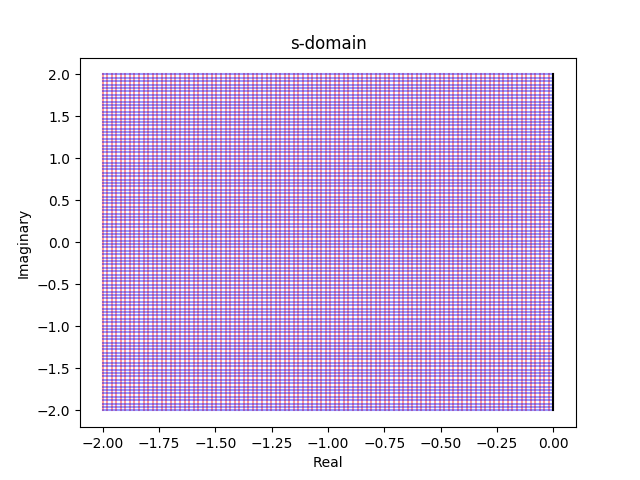
\includegraphics{Figures/s_grid.png}
 \caption{A grid in the s-domain}
 \label{fig:s_grid}
\end{figure}{}
\begin{figure}
 \centering
 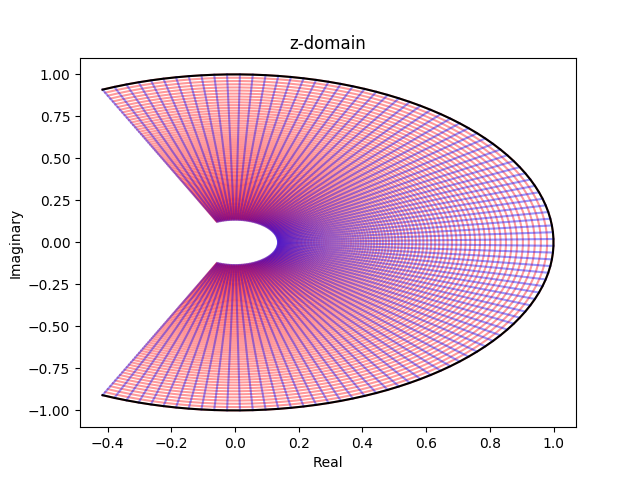
\includegraphics{Figures/z_grid.png}
 \caption{The same grid in the z-domain, sampled with a sampling period of 1 time-unit. The black line on the right side is the stability-border}
 \label{fig:z_grid}
\end{figure}{}


\begin{figure}
 \centering
 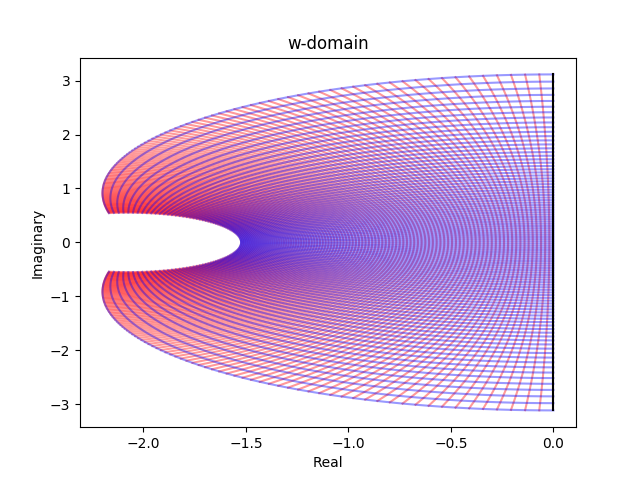
\includegraphics{Figures/w_grid.png}
 \caption{Grid in w-domain, with a sampling period of 1 time-unit}
 \label{fig:w_grid}
\end{figure}{}
As shown in \cref{fig:s_grid} and \ref{fig:w_grid}, there can be quite a bit of distortion between the s-domain and the w-domain. But the differences are rather small for poles closer to the origin. So, intuitively, the w-domain behaves more like the s-domain when the system gets closer to the stability-border, which should hopefully make it more suited for stability-analysis. 

In order to prove that the stability regions are what we say they are, we will have to do some substitutions. First, since $z = e^{s T_s}$, the only requirement is to divide it into two and observe that 
\begin{equation}
 z = e^{\Re{(s )T_s}}e^{\Im{(s )T_s}}
\end{equation}{}
Since an imaginary exponent does not change the absolute value, only the complex angle, the real part of s directly translates to the amplitude of z. Real parts less than 0, gives amplitudes less than 0. This means that the stability region will be inside the unit circle. 


Similarly, $z$ can be represented as $z = r\cdot e^{j\Theta}$. If it is put into the equation for $w$, the resulting expression becomes:

\begin{equation}
 w = \frac{2}{T}\frac{r e^{j \Theta}-1}{re^{j \Theta}+1}
\end{equation}{}
After using Euler's formula, we get: 
\begin{equation}
 w = \frac{2}{T_s} \frac{(r^2 -1) + j( 2\sin{\Theta}) }{1+ r^2 + 2r \cos{\Theta}}
\end{equation}{}

Since the denominator is real, the real part of $w$ is described entirely by $\frac{r^2-1}{1+r^2 + 2 r cos (\Theta)}$. As a result, when $r<1$, then $\Re{(w)} < 0$. Also, worth noting is that as long as $\Theta =0$, the $w$ will never go beyond $-\frac{2}{T_s}$. This means that purely real eigenvalues will never go beyond the Nyquist-frequency, even though they may have faster dynamics in the s-domain. Also, if $\Theta =\frac{\pi}{2}$, and $r=1$, then, the denominator will be equal to 0. By L'Hôpital's rule, the resulting amplitude will be $\infty$. This means that oscillations near the Nyquist-frequency will potentially be mapped far away from where a similar point would have been in the s-domain. This helps to highlight one of the weaknesses of the w-transform. If a mode is very close to the Nyquist-frequency if will become more difficult to analyze. But preferably, all modes that might cause instability should be below the Nyquist-frequency. But, in practice, in order to avoid the issues of sampling, it is normal to have a sampling-rate that is between $\frac{1}{2}$ and $\frac{1}{5}$ of the Nyquist-frequency. The advantages of a high sampling-frequency can be seen in \cref{fig:dif_s_and_w}. As a result of the high sampling-rate, the differences will usually not be that large.


\begin{figure}
 \centering
 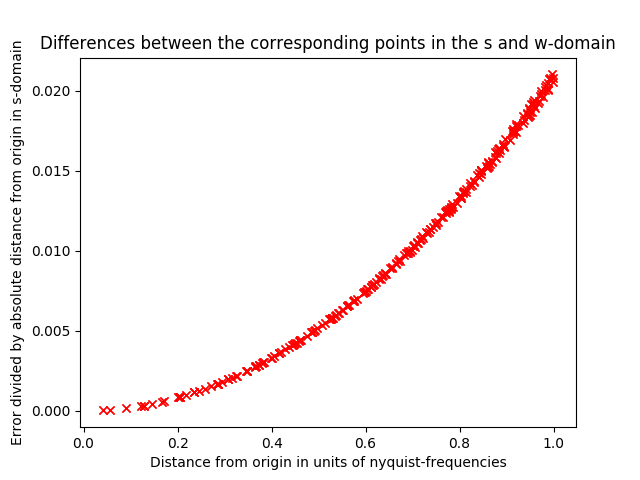
\includegraphics{Figures/differences_in_well_behaved_region.png}
 \caption{The difference between a point in the s-domain and in the w-domain is quite good below the Nyquist-frequency, but becomes worse quickly}
 \label{fig:dif_s_and_w}
\end{figure}
\todo[inline]{Nyquist ofte mellom 1/5 og maks til 1/2 av Nyquist (eller 1/10 og 1/20)}
\noindent

Finally, the last useful characteristic of the w-transform is that, unlike the z-transform, the placement of the poles are not as affected by the sampling-frequency as the z-transform. In the z-transform, a pole at $\lambda_i$, at a sampling-period $T_s$, will be mapped to the same point as a pole at $2\lambda_i$ if the sampling-period is halved to $\frac{T_s}{2}$. As long as the sampling-rate is so high that a pole is within the somewhat linear part of the w-domain, it will not change a position based on the sampling-frequency. This may make the analysis a bit more intuitive. 
\chapter{A linearized model of the grid and controller}
\label{chp:linearize_the_system}
Setting up the linear system can be cumbersome job, and has to be done in two parts if the goal is to get a solution that is as exact as possible. First, the continuous system has to be linearized and solved exactly, and then, we must assume that all inputs from the controller are zero-order hold elements. If they are, it is possible to get an exact solution of the dynamics in the z-domain. In order to linearize the continuous system, the easiest way to do it is to write it in the dq-reference frame. The resulting equations for one VSC are: 

For the filter-side of the converter
\begin{align}
 \frac{d}{dt}&\Vec{v_o} = \frac{\omega_b}{c_f}\Vec{i_{cv}} - \frac{\omega_b}{c_f}\Vec{i_o} - j\cdot\omega_b \omega_g \Vec{v_o}\\
 \frac{d}{dt}&\Vec{i_{cv}} = \frac{\omega_b}{l_f}\Vec{v_{cv}} - \frac{\omega_b}{l_f}\Vec{v_o} -\omega_b \left( \frac{r_{l_f}}{l_f} + j\cdot \omega_g \right)\Vec{i_{cv}}\\
 \frac{d}{dt}&\Vec{i_o} = \frac{\omega_b}{l_g}\Vec{v_{o}} - \frac{\omega_b}{l_g}\Vec{v_g} -\omega_b \left( \frac{r_g}{l_g} + j\cdot \omega_g \right)\Vec{i_o}\\
\end{align}{}

If $\Vec{v_g}$ is constant, it can be considered as an input. If not, the rest of the grid has to be added as states and solved for as well. 

For the DC-side of the converter
\begin{align}
 \frac{d}{dt}&v_{dc} = \frac{\omega_b}{c_{dc}}i_{dc,s} - \frac{\omega_b}{c_{dc}}i_{dc}\\
 \frac{d}{dt}&i_{dc,s} = \frac{\omega_b}{l_{dc}}v_{dc,s} -\frac{\omega_b}{l_{dc}}v_{dc} - \omega_b \frac{ r_{dc}}{l_{dc}}i_{dc,s} \\
\end{align}{}


The system will have to be linearized around some stationary operating point. This means that $\Vec{x^{true}} = \Vec{x_0}+ \Vec{x}$. The vector $\Vec{x}$ will be used to reffer to the deviation of the states from the stationary operating point.Because a linear operating point is suposed to mean that $0 = \Vec{A}\Vec{x_0} + \Vec{B}\Vec{u_0}$, the states of the linear system can be written as:

\begin{equation}
\Vec{x}_{cont}=
\begin{bmatrix}
 \Delta v_{o,d}\\
 \Delta v_{o,q}\\
 \Delta i_{cv,d}\\
 \Delta i_{cv,q}\\
 \Delta i_{o,d}\\
 \Delta i_{o,q}\\
 \Delta v_{dc} \\
 \Delta i_{dc,s}
\end{bmatrix}{}
, \Vec{u}_{cont}
\begin{bmatrix}
 \Delta v_{cv,d}\\
 \Delta v_{cv,q}\\
 \Delta v_{g,d}\\
 \Delta v_{g,q}\\
 \Delta i_{dc}\\
 \Delta v_{dc,s}\\
\end{bmatrix}{}
\end{equation}{}
Where the $\Delta$s mean that the variables signify the difference from the linear operating point.
\begin{equation}
\Dot{\Vec{x}}_{cont}= 
\Vec{A}_{cont} \Vec{x}_{cont} + \Vec{B}_{cont}\Vec{u}_{cont}
\end{equation}{}
The system-matrix is so big that it does not fit on one page, so we have to define 
\begin{equation}
 \Vec{A}_{cont}= 
 \begin{bmatrix}
 \Vec{A}_{cont, 1} & \Vec{A}_{cont,2}
 \end{bmatrix}
\end{equation}
Where: 
\begin{equation}
 \Vec{A}_{cont,1}=
 \begin{bmatrix}
 0 & \omega_b\omega_g & \frac{\omega_b}{c_f} & 0 \\
 -\omega_b\omega_g & 0 & 0 & \frac{\omega_b}{c_f} \\
 -\frac{\omega_b}{l_f}&0 &- \omega_b\frac{r_{l_f}}{l_f} & \omega_b\omega_g \\
 0 &-\frac{\omega_b}{l_f} &-\omega_b\omega_g & -\omega_b\frac{r_{l_f}}{l_f} \\
 \frac{\omega_b}{l_g} & 0 & 0 & 0 \\
 0 & \frac{\omega_b}{l_g} & 0 & 0 \\
 0 &0 &-\frac{\omega_b}{c_{dc}}\frac{v_{cv,d,0}}{v_{dc,0}}&-\frac{\omega_b}{c_{dc}}\frac{v_{cv,d,0}}{v_{dc,0}}\\
 0 &0 &0 &0 \\
 
 \end{bmatrix}{}
\end{equation}{}
\begin{equation}
 \Vec{A}_{cont,2}=
 \begin{bmatrix}

& -\frac{\omega_b}{c_f} & 0 & 0 & 0\\
& 0 & -\frac{\omega_b}{c_f} & 0 & 0 \\
& 0 & 0 & 0 & 0\\
& 0 & 0 & 0 & 0 \\
& -\omega_b\frac{r_g}{l_g} & \omega_b \omega_g & 0 & 0\\
& -\omega_b \omega_g & -\omega_b\frac{r_g}{l_g} & 0 & 0\\
&0 &0 & \omega_b \frac{i_{cv,d,0}v_{cv,d,0} + i_{cv,q,0}v_{cv,q,0} }{v_{dc,0}^2} &\frac{\omega_b}{c_{dc}} \\
&0 &0 &- \frac{\omega_b}{l_{dc}} & - \omega_b \frac{r_{dc}}{l_{dc}} \\
 
\end{bmatrix}{}
\end{equation}{}
The matrix for the input can be written as: 
\begin{equation}
 \Vec{B}_{cont} = 
 \begin{bmatrix}
 \frac{\omega_b}{l_f} & 0&0&0&0&0\\
 0 & \frac{\omega_b}{l_f}&0&0&0&0\\
 0 &0 &0&0&0&0\\
 0 &0 &0&0&0&0\\
 0 &0 &-\frac{\omega_b}{l_g} & 0&0&0\\
 0 &0 &0&-\frac{\omega_b}{l_g}&0&0\\
 0 &0 &0&0& -\frac{\omega_b}{c_{dc}} & 0\\
 0 &0 &0&0& 0 & \omega_b \frac{r_{dc}}{l_{dc}}\\
 
 
 \end{bmatrix}{}
\end{equation}{}{}

But the controller only has two degrees of freedom in controlling $v_{cv,d}$ and $v_{cv,q}$ and the current $i_{dc}$ is limited by the power-balance. The resulting $\Vec{B}$-matrix that represents how the controller can influence the system becomes somewhat simpler. 

The controller will always be affected by a power-balance between the DC and the AC-side.
\begin{equation}
 v_{dc} i_{dc} = v_{cv,d} i_{cv,d} + v_{cv,q}i_{cv,q}
\end{equation}{}
The voltage $v_{dc}$ must be the same as the voltage over the capacitor, since there are no components between the input-voltage of the \gls{VSC} on the DC-side and the capacitor $C\gls{_dc}$. Also, if the constraints given by the power-balance are linearized, the resulting equation becomes: 
\begin{equation}
 i_{dc,cv} = \frac{v_{cv,d}i_{cv,d} + v_{cv,q}i_{cv,q}}{v_{dc}}
\end{equation}{}
The resulting differential equation for the voltage $v_{dc}$ gives 
\begin{equation}
 \dot{v}_{dc} = \frac{\omega_b}{c_{dc}} \left( i_{dc,s} - \frac{v_{cv,d}i_{cv,d} + v_{cv,q}i_{cv,q} }{v_{dc}} \right) 
\end{equation}{}
When this is linearized around some operating point $\Vec{x}_0$, the result will be: 

\begin{dmath}
 \dot{v}_{dc} = \Delta \dot{v}_{dc} \approx \frac{\omega_b \Delta i_{dc,s}}{c_{dc}} - \frac{\omega_b}{c_{dc}}\left( \frac{v_{cv,d,0} \Delta i_{cv,d}}{v_{dc,0}} + \frac{i_{cv,d,0} \Delta v_{cv,d}}{v_{dc,0}} - \frac{i_{cv,d,0}v_{cv,d,0}}{\left(v_{dc,0}\right)^2}\Delta v_{dc,0}\\
 + \frac{v_{cv,q,0} \Delta i_{cv,q}}{v_{dc,0}} + \frac{i_{cv,q,0} \Delta v_{cv,q}}{v_{dc,0}} - \frac{i_{cv,q,0}v_{cv,q,0}}{\left(v_{dc,0}\right)^2}\Delta v_{dc,0}
 \right)
\end{dmath}{}





% This means that the voltages $v_{cv}$ will also affect the DC-current when the system is linearized. 
After extracting the terms relating $v_{cv,d}$ and $v_{cv,q}$, the matrix $\Vec{B_s}$ can be found. (The effects of the power-balance were already added to $\Vec{A_{cont}}$) 
\begin{equation}
 \Vec{B_s} = 
 \begin{bmatrix}
 \frac{\omega_b}{l_f} & 0\\
 0 & \frac{\omega_b}{l_f}\\
 0&0\\
 0&0\\
 0&0\\
 0&0\\
 -\frac{\omega_b}{c_{dc}}\frac{i_{cv,d,0}}{v_{dc,0}}&-\frac{\omega_b}{c_{dc}}\frac{i_{cv,q,0}}{v_{dc,0}}\\
 0&0\\
 \end{bmatrix}{}
\end{equation}{}

To get more consistent notation, we also say that
\begin{equation}
 \Vec{A_s} = \Vec{A_{cont}}
\end{equation}
If the converter is a part of a larger grid, then $v_g$ has to be replaced with a state from the grid, and all continuous components simply have to be solved in the same manner, but overall, the method will not change. Since it is assumed that all actuators on the system are zero-order hold elements, it is possible to make a new state $x_z$, which contains $x_{cont}$, as well as all internal states in the controller, and the delayed inputs from the controller to the system. The discretised system can be written as: 
\begin{equation}
 z {x}_z = 
 \begin{bmatrix}
 e^{\Vec{A}_s T_s} & \Vec{A}_s^{-1}( e^{\Vec{A}_s T_s} - \Vec{I}) \Vec{B_s} & \Vec{0}\\
 \Vec{K_1} & \Vec{0} & \Vec{K_2} \\
 \Vec{K_3} \hat{T_s} & 0 & \Vec{K_4} \hat{T_s}
 \end{bmatrix}{}
 x_z
 \label{eq:A_z}
\end{equation}{}
Where $\Vec{K_1}$ is the matrix representing how the measured states will affect the output at the next timestep. $\Vec{K_2}$ represents how the internal states affect the output of the controller. $\Vec{K_3}$ and $\Vec{K_4}$ shows how the internal states are affected by the measured states and the internal states respectively. $\hat{T_s}$ represents the estimated sampling, frequency, is assumed to be the same as $T_s$, but may differ from the real one. Since the controller is sampled, the inputs will also be delayed before affecting the system. As a result, $\Vec{x_z}$ can be divided into three parts. 

\begin{equation}
 \Vec{x_z} = 
\begin{bmatrix}
 \Vec{x_{cont}} \\
 \Vec{x_{u}} \\
 \Vec{x_{controller}} \\
\end{bmatrix}{}
\end{equation}{}

When looking at the state-space representation in \cite{Suul_paper_1}, the inputs to the system can be seen directly in the state-space, resulting in a vector.
\begin{equation}
 \Vec{x_u} = 
 \begin{bmatrix}
 v_{cv,d}\\ v_{cv,q}\\
 \end{bmatrix}{}
\end{equation}{}
The simplest controller is a current-controller without active damping. To implement this, the internal states of the controller need to be at contain the following parameters: 
\begin{equation}
 \Vec{x_{controller}} = 
 \begin{bmatrix}
 \delta\theta_{PLL} \\ \gamma_d \\ \gamma_q \\ v_{PLL,d} \\ v_{PLL,q} \\ \epsilon_{PLL} \\
 \end{bmatrix}{}
\end{equation}{}

$\delta\theta_{PLL}$ is the error in the estimate of the grid-phase that the \gls{PLL} gives out. $\gamma_d$ and $\gamma_q$ are the integrators used PI current-controller. $v_{PLL, d}$, $v_{PLL, q}$ are the internal states of the low-pass filter used by the \gls{PLL}, and finally, $\epsilon_{PLL}$ is the integrator- used by the PI-controller in the \gls{PLL}



Since all these states are integrators of the deviation from some kind of reference, the stationary reference point should mean that $\Vec{x}_{controller, 0} =0$. So there is no need for using terms using $\Delta$ here. 

\section{Describing the internal states in a current-controller}

Since no more information is given than the measured data-points, the controller will simply be implemented by first-order forward Euler. 

Depending on the type of controller, the states in $\Vec{x_{controller}}$, as well as the control-laws that are described in the $\Vec{K}$-matrices may be replaced by something else. But, in this case, we will simply use a current controller without active damping, but with a decoupling-term between the two parts of $\Vec{v}\gls{_cv}$. The resulting matrices will be:


\begin{equation}
 \Vec{\dot{x}}_{controller}=
 \begin{bmatrix}
 \frac{\omega_b k_{p,PLL}}{v_{o,0}} v_{PLL, q} + \omega_b k_{i,PLL} \epsilon_{PLL}\\
 - i_{cv,d} + i_{cv,d}^* \\
 - i_{cv,q} + i_{cv,d}^* \\
 \omega_{LP,PLL}(v_{o,d} - v_{PLL,d})\\
 \omega_{LP,PLL}(v_{o,q} - v_{PLL,q})\\
 \frac{1}{v_{o,d,0} }v_{PLL,q}\\
 \end{bmatrix}{}
\end{equation}{}

\begin{equation}
 \Vec{K_3} = 
 \begin{bmatrix}
 0 &0&0&0 &0 &0&0&0\\
 0 & 0 & -1&0 &0&0&0&0\\
 0 & 0 & 0 & -1& 0 &0&0&0\\
 \omega_{LP, PLL} & 0 & 0&0 &0&0&0&0\\
 0 & \omega_{LP, PLL} &0 &0&0&0&0&0\\
 0 &0&0&0&0 &0&0&0\\
 \end{bmatrix}{}
\end{equation}{}

\begin{equation}
 \Vec{K_4} = 
 \begin{bmatrix}
 0 &0&0&0 &0 &0&\frac{\omega_b k_{i,PLL}}{v_{o,d,0}}&\omega_b k_{i,PLL}\\
 0&0&0&0&0&0&0&0\\
 0&0&0&0&0&0&0&0\\
 0 & 0 & 0&0 &0&-\omega_{LP, PLL}&0&0\\
 0 & 0&0 & 0&0 &0&-\omega_{LP, PLL}&0\\
 0 & 0 &0 &0&0&0&\frac{1}{v_{o,d,0}}&0
 \end{bmatrix}{}
 \end{equation}{}
As a result, the reference voltage will become


\begin{equation}
 z\Vec{x_u}= 
 \begin{bmatrix}
 -k_{pc} i_{cv,d} + \omega_g l_f i_{cv,q} + k_{ic} \gamma_d 
 -l_f \frac{k_{p,PLL}i^*_{cv,q,0}}{v_{o,d,0}} v_{PLL, q} - l_f k_{i,PLL} i_{cv,q,0}^* \epsilon_{PLL } \\
 -k_{pc} i_{cv,q} - \omega_g l_f i_{cv,d} +k_{ic} \gamma_q +
 l_f \frac{k_{p,PLL}i^*_{cv,q,0}}{v_{o,d,0}} v_{PLL, q} + l_f k_{i,PLL} i_{cv,q,0}^* \epsilon_{PLL }\\
 \end{bmatrix}{}
\end{equation}{}

Because of this, the matrices describing the two values in $v_{cv}$ become:

\begin{equation}
 \Vec{K_1} = 
 \begin{bmatrix}
 0 & 0& -k_{pc} & \omega_g l_f & 0 & 0 & 0&0\\
 0 & 0& -\omega_g l_f &k_{pc} & 0 & 0 & 0&0
 \end{bmatrix}
\end{equation}{}
\begin{equation}
\Vec{K_2} =
\begin{bmatrix}
 0&k_{ic}&0 & 0 & -l_f \frac{k_{p,PLL}i^*_{cv,q,0}}{v_{o,d,0}}&l_f k_{i,PLL}i^*_{cv,q,0}\\
 0& 0&k_{ic}&0 & l_f \frac{k_{p,PLL}i^*_{cv,q,0}}{v_{o,d,0}}&l_f k_{i,PLL}i^*_{cv,q,0}
\end{bmatrix}
\end{equation}{}

\todo[inline]{Explain the assumption that angular error has to be treated as a continuous state (Or does it?) }


\chapter{Contribution}
\label{chp:new_findings}
\section{Transforming a MIMO-system into the system into the w-domain}

As described in \cref{chp:w_transformation}, the eigenvalues of a system can be written in the w-domain as: 
 
\begin{equation}
 w\Vec{x} = \Vec{A}_w\Vec{x} + \Vec{B}_w\Vec{u}
 \label{eq:MIMO_in_w}
\end{equation}{}

If the system is on this form given in \cref{eq:MIMO_in_w}, it will be stable if all eigenvalues of $\Vec{A_w}$ are in the left half-plane. 

By using the derivative of the eigenvalues of $\Vec{A_w}$, it is possible to say something about how sensitive the system is to changes in the different parameters that define $\Vec{A_w}$. Consequently, the derivative will be able to tell how plausible it is that some of the eigenvalues might end up in the right half-plane. This can be very useful when estimating the robustness against modeling errors. 

Ideally, we want to find out as precisely as possible how much the eigenvalues change if we are slightly wrong about the parameters in our physical system. The derivatives of $\lambda$ will not be able to tell exactly at what point an eigenvalue will cross over to the right half-plane, but for small changes, the derivative is often a decent approximation. But in order to find the derivative in the w-domain, we will have to step through the entire transformation of how we got from the time-domain all the way to the w-domain. 

How to find the derivative of an eigenvalue was described in \cite{Suul_eigenvalue_presentation}, but will be re-elaborated here. 

In order to find the derivative of an eigenvalue $\lambda_i$, the vectors $\phi_i$ and $\psi_i$ are needed. $\phi_i$ and $\psi_i$ have to be eigenvectors and eigencolumns corresponding to an eigenvalue $\lambda_i$. So they have to fulfil
\begin{equation}
 \Vec{A}\phi_i = \lambda_i \phi_i
\end{equation}{}
\begin{equation}
\psi_i\Vec{A}= \lambda_i \psi_i
\end{equation}{}
If $\psi_i$ and $\phi_i$ also satisfy the requirement that 
\begin{align}
 \psi_i \phi_j = 0 \forall i \neq j \\
 \psi_i \phi_i = 1 \forall i
\end{align}{}
Then
\todo[inline]{Finn en ordentlig refferanse som beskriver dette ordentlig, eller forklar det selv ( Virker vanskelig ) }
\todo[inline]{Uttrykket for endringen i eigenverdien må endres}
\begin{equation}
 \frac{d \lambda_{w,i}}{d \rho} = \frac{1}{|\psi_i \phi_i|} \psi_i \frac{d \Vec{A_w}}{d \rho }\phi_i 
\end{equation}{}
In order to find the sensitivity of the eigenvalues with respect to a parameter in the physical system, it is necessary to use the chain rule through every step that was done in the transformation, until we reach the step $\frac{d \Vec{A_s}}{d \rho}$, or $\frac{d \Vec{B_{cont}}}{d \rho}$, which can be differentiated directly. 


As shown in \cref{sec:Transforming_from_z_to_w}, the transformation from the z-domain to the w-domain is: 

\begin{equation}
 \Vec{A}_w = \frac{2}{T} \left(\Vec{I} - 2( \Vec{I}+\Vec{A}_z)^{-1}\right)
\end{equation}{}

We use the trick from \cite{Matrix_differentiation_source}, the inverse of a matrix $\Vec{A}$ can be found by: 

\begin{equation}
 \frac{d \Vec{I}}{d \rho} = \frac{d ((\Vec{A})(\Vec{A})^{-1}}{d \rho} = 0
\end{equation}{}

\begin{equation}
 \frac{d (\Vec{A})(\Vec{A})^{-1}}{d \rho} = 
 \frac{d (\Vec{A})}{d \rho} (\Vec{A})^{-1} +
 (\Vec{A})\frac{d (\Vec{A})^{-1}}{d \rho}
\end{equation}{}

Which gives: 
\begin{equation}
 \frac{d (\Vec{I}+\Vec{A})^{-1}}{d \rho} = - (\Vec{I}+\Vec{A})^{-1}\frac{d (\Vec{A})}{d \rho} (\Vec{I}+\Vec{A})^{-1} 
\end{equation}{}

And when applying that to the differentiation of $\Vec{A}_w$
\begin{equation}
 \frac{d \Vec{A}_w}{d \rho} = \frac{4}{T} (\Vec{I}+\Vec{A}_z)^{-1}\frac{d (\Vec{A}_z)}{d \rho} (\Vec{I}+\Vec{A}_z)^{-1}
\end{equation}{}
But this is where the fun ends. $A_z$ comes from a combination several different submatrices with different dynamics. Luckily, when differentiating a matrix with respect to a scalar, the sub-matrices can be differentiated independantly. If the impulse-response of $\Vec{A_s}$ is defined as $\gls{impulse_resp}\gls{_s}$, step-response is defined as $\gls{step_resp}\gls{_s}$, then the matrix $\Vec{A_z}$ can be defined as: 

\begin{equation}
 \Vec{A_z} = 
 \begin{bmatrix}
 \gls{impulse_resp}\gls{_s} & \gls{step_resp}\gls{_s}\Vec{B_s} & \Vec{0}\\
 \Vec{K_1} & \Vec{0} & \Vec{K_2}\\
 \Vec{K_3} & \Vec{0} & \Vec{K_4}
 \end{bmatrix}{}
\end{equation}{}

All matrices $\Vec{K_i}$ can be differentiated directly and should not result in any problems. Meanwhile, the impulse-response is always:
\begin{equation}
 \gls{impulse_resp} = e^{\Vec{A} T_s}
\end{equation}
The step-response is allways defined, but if $\Vec{A_s}$ is invertible, then it can be written as in \cref{eq:easy_step_resp}. If not, it has to be found as in \cref{sec:solving_for_uninvertible_matrices}
\begin{equation}
 \gls{step_resp}_s = \Vec{A_s}^{-1}\left( e^{\Vec{A_s}T_s} - \Vec{I}\right)
 \label{eq:easy_step_resp}
\end{equation} 


% As long as $\Vec{A}_s$ has full rank, its inverse can be differentiated like what had been done in the previous section. If $\Vec{A_s}$ does not have full rank, it is still possible to find out how the system responds to constant inputs, and it may still be possible to differentiate the expression under certain conditions, as will be discussed in \cref{sec:differentiating_step_response_from_input}. But, since electrical grids usually are passive, it is quite likely that $\Vec{A_s}$ has an empty null-space. 


During this project, no general method was found for differentiating $\Vec{e^{A_s T_s}}$ with respect to $\rho$
% \begin{equation}
% \frac{d }{d \rho} \left( \Vec{e^{A_s T_s}} \right)
% \end{equation}{}
There might not exist a way to perform the differentiation. But there is still be hope if our goal just is to get an upper bound on the sensitivity. 

\noindent 


The matrix $e^{\Vec{A_s} t}$ is defined as 
\begin{equation}
 e^{A_s t} = I + At + \frac{A^2 t^2}{2!} + ... + \frac{A^n t^n}{n!} + ...
\end{equation}{}

During this project, no better method was found for differentiating Taylor-series. As a result, we simply use the product rule, which gives. 

\begin{equation}
 \frac{d (\Vec{A})^n}{a_{i,j}} = \sum_{k=1}^{n}\Vec{A}^{k-1} \frac{d \Vec{A}}{d a_{i,j}} \Vec{A}^{n-k}
\end{equation}{}

Since it is not possible to compute such an infinite sum numerically, it is necessary to make an approximation by dropping the terms after a certain point.

\begin{equation}
 \frac{d\hat{\gls{impulse_resp}}}{d\rho} = \frac{d}{d \rho} \sum_{i=0}^{N} \frac{A^i t^i}{i!}
\end{equation}

The step-response suffers from similair problems. If $\Vec{A_s}$ is invertible, the best estimate can be given by: 
\begin{dmath}
 \hat{\gls{step_resp}}_s = \Vec{A_s}^{-1}\frac{d\hat{\gls{impulse_resp}}}{d\rho} - \Vec{A_s}^{-1}\frac{d A_s}{d\rho}\hat{\gls{step_resp}}_s
\end{dmath}
If not, the method from \cref{sec:differentiating_step_response_from_input}, has to be used instead, if the conditions are met.
The error bound is discussed in \cref{sec:how_bad_can_it_go}. We define the estimated derivative of a matrix $\frac{\Vec{A}}{d \rho}$ as a matrix $\Delta \Vec{A}$. The resulting approximation for the derivative of $\frac{d \Vec{A_z}}{d \rho}$ becomes: 
\begin{equation}
 \Delta\Vec{A_z} = 
 \begin{bmatrix} 
 \frac{d \hat{\gls{impulse_resp}}_s}{d \rho} & \frac{d \hat{\gls{step_resp}}_s}{d \rho}\Vec{B} + \gls{step_resp}_s\frac{d \Vec{B_s}}{d \rho} & 0\\
 \frac{d \Vec{K_1}}{d \rho} & 0 & \frac{d \Vec{K_2}}{d \rho}\\
 \frac{d \Vec{K_3}}{d \rho} & 0 & \frac{d \Vec{K_4}}{d \rho}
 \end{bmatrix}
 \label{eq:approx_dA_z}
\end{equation}{}

The the derivatives of the sub-matrices $\frac{d \Vec{K_1}}{d \rho} $, $ \frac{d \Vec{K_2}}{d \rho}\frac{d \Vec{K_3}}{d \rho} $, $ \frac{d \Vec{K_4}}{d \rho}$ can all be found directly, and will usually be equal to 0.


The explicit solution for $\hat{\gls{impulse_resp}}_s$ is: 
\begin{equation}
 \frac{d \hat{\gls{impulse_resp}}_s}{d \rho} =
 \sum_{n=0}^N \sum_{k=1}^n \frac{(T_s)^n}{n!} \Vec{A_s}^{k-1} \frac{d \Vec{A_s}}{d \rho} \Vec{A_s}^{n-k}
\end{equation}


Electrical circuits that are only made of resistors, inductors capacitors, and voltage/current-sources without any state feedback are always passive. For linear systems, this will mean that all states will go towards 0. As a result, $\Vec{A_s}$ must have full rank, which means $\Vec{A_s}$ is invertible. If there are more converters or generators in the grid, they may cause issues, but it is quite unlikely. 


After the long process of differentiating the expression, we can avoid the almost impossible task of having to symbolically find the values in the w-domain, but it did cost some precision. Since we were unable to find the actual derivative of the matrix $\Vec{e^{At}}$, even though the rest of the matrix $\Vec{A_z}$ was found exactly. 


Finally, after approximating the derivative of $\frac{d e^{\Vec{A}t}}{d a_{i,j}}$, we can look at how the different elements in $\Vec{A_s}$ and $\Vec{B_s}$ can change, depending on the changes in parameters. If this is multiplied by the expected difference between the real and the estimated value of the components, it will be possible to get an idea of how robust the system is. Actual estimates of the robustness will most likely also require some statistical analysis. 


\section{Giving upper bounds to the error}
\label{sec:how_bad_can_it_go}
We were not able to differentiate $\frac{d e^{A(x) T_s}}{d \rho}$, so now it will be necessary to give an upper bound to how far the estimated eigenvalues can be from the real ones. In order to do that, it will be necessary to have an upper bound for how much the eigenvalues might change because of the error. This can be done by using matrix-norms, as seen in \cite{Triangle_inequality_source} and \cref{sec:induced_matrix_norms}. Additionally, it will also be necessary to traverse backwards through the transformations when taking the norm between the real derivative of the eigenvalues, and the estimated ones, similar to how it was done when differentiating the eigenvalues. 

\subsection{An upper bound on the error of \texorpdfstring{$\frac{d e^{\Vec{A}t}}{d\rho}$}{TEXT}}
\label{sec:upper_bound_norm_eAt}
In order to estimate the error, we will define the error of the simplified Taylor-series as: 
\begin{equation}
 \tilde{\mathbb{A}} = \sum_{i = N}^\infty \Vec{A}^{i}\frac{\left(T_s \right)^i }{i!}
\end{equation}
As a result: 
\begin{equation}
 \frac{d\tilde{\mathbb{A}}}{d\rho} = \sum_{i=N}^\infty \sum_{k=1}^i \Vec{A}^{k-1}\frac{d \Vec{A}}{d \rho}\Vec{A}^{i-k}\frac{\left(T_s \right)^i }{i!}
\end{equation}

We will use the fact that $\norm{\Vec{AB}}\leq \norm{\Vec{A}} \cdot \norm{\Vec{B}}$ for all operator norms, as mentioned in \cite{Triangle_inequality_source} and shown in \cref{sec:induced_matrix_norms}. As a result of this inequality, an upper vound can be given for $\frac{d\tilde{\mathbb{A}}}{d\rho}$
\begin{equation}
 \norm{\frac{d}{d\rho} \sum_{n=N}^\infty \frac{T_s^n}{n!}\Vec{ A}^n} \leq \sum_{n=N}^\infty \frac{T_s^n}{n!} n\left( \norm{\frac{d\Vec{ A}}{d x}} \cdot \norm{\Vec{ A}}^{n-1}\right)
\end{equation}{}

$\norm{\Vec{ A}}$ and $\norm{\frac{d\Vec{ A}}{d x}}$ can both be calculated, while $T_s$ is known beforehand. Therefore, the series may be upper bounded by: 

\begin{equation}
 \norm{\frac{d}{d\rho} \sum_{n=N}^\infty \frac{T_s^n}{n!}\Vec{ A}^n} \leq \frac{\norm{\frac{d\Vec{ A}}{d x}}}{|T_s|} \left( e^{\norm{\Vec{A}} T_s} - \sum_{n=0}^{N-1} \frac{\left(\norm{\Vec{A}} T_s \right)^n}{n!}\right)
 \label{eq:upper_bound_deAt}
\end{equation}{}

In this project, we will be using the $\mathcal{L}_1$ operator norm, since it is easy, and allows for some simplifications when calculating norms of matrices when the norms of the submatrices are known. But the analysis still holds for other operator norms as well. 

\subsection{An upper bound for the derivative of \texorpdfstring{$\lambda$}{TEXT}}
Given a perfect estimate $\Delta\Vec{A_w^*}$ of $\frac{d \Vec{A_w}}{d\rho}$, the eigenvalues can be found exactly. 
\begin{equation} 
 \frac{d \lambda_{i}}{d \rho} = \frac{1}{|\psi\phi|} \phi_i \Delta\Vec{A_w^*} \phi_i 
\end{equation}{}
\todo[inline]{Sørg for at phi og psi er riktig transponert}

The perfect estimate can be divided int two parts 
\begin{equation}
 \Delta\Vec{A_w^*} = \Delta\Vec{A_w} + \tilde{\Delta\Vec{A_w}}
\end{equation}
Where $\Delta\Vec{A_w}$ is our estimate of $\frac{d \Vec{A_w}}{d\rho}$, and $\tilde{\Delta\Vec{A_w}}$ is the error. 
The estimates are given by the equation: 
\begin{equation}
 \Delta\Vec{A_w^*} = - ( \Vec{I}+\Vec{A}_z)^{-1} \Vec{\Delta A_z^{*}} ( \Vec{I}+\Vec{A}_z)^{-1}
\end{equation}{}

As a result, the two matrices can be described by the estimate of $\Delta\Vec{A_w}$ and the error. 
\begin{align}
 \Delta\Vec{A_w} = - ( \Vec{I}+\Vec{A}_z)^{-1} \Vec{\Delta A_z}( \Vec{I}+\Vec{A}_z)^{-1}\\
 \Delta\Vec{\Tilde{A}_w} = - ( \Vec{I}+\Vec{A}_z)^{-1} \Vec{\Delta \Tilde{A}_z}( \Vec{I}+\Vec{A}_z)^{-1}
\end{align}{}

$\Vec{\Delta A_z}$ is given by \cref{eq:approx_dA_z}, which has an exact solution. $\Vec{\Delta \Tilde{A}_z}$ is the differentiation of the remaining terms and must be given an upper bound instead. 


In order to give an upper bound to the change that results form $\Vec{\Delta \Tilde{A}_z}$, it is possible to use the submultiplicative property of operator norms. As explained in \cite{Triangle_inequality_source}, and re elaborated in \Cref{sec:induced_matrix_norms}, any incuced operator norm will satisfy.
\begin{equation}
 ||\Vec{AB}|| \leq ||\Vec{A}|| \cdot ||\Vec{B}|| \quad \forall \Vec{A}, \Vec{B} \in \Re^{n \times n}
 \label{eq:submultiplicativity}
\end{equation}

For simplicity, it is possible to just use the $\mathcal{L}_1$-norm, which is given by: 

\begin{equation}
 \norm{\Vec{A}}_1 = \max_j \sum_{i}\left|\Vec{A}_{i,j}\right|
\end{equation}

\todo[inline]{Sørg for at det some er før og etter her passer sammen}
\begin{equation}
 \norm{ \Vec{ \Delta \Tilde{A}_w} } \leq \norm{( \Vec{I}+\Vec{A}_z)^{-1}} \cdot \norm{\Vec{\Delta \Tilde{A}_z}} \cdot \norm{( \Vec{I}+\Vec{A}_z)^{-1}}
\end{equation}{}

The norm of $\norm{( \Vec{I}+\Vec{A}_z)^{-1}}$ can be found easily. So the only issue is $\norm{\Vec{\Delta \Tilde{A}_z}}$, which has several sub-matrices where $e^{\Vec{A_s}T_s}$ is a factor. 

If an upper bound of a matrix-norm has to be given, based on the norm of the sub-matrices, it will depend on the type of norm. When using the $\mathcal{L}_1$-norm, an upper bound can be found by treating  the norms of the sub-matrices  as elements instead, i.e.

\begin{equation}
 \norm{\begin{bmatrix}
 \Vec{A_{1,1}} & \cdots & \Vec{A_{1,n}}\\
 \vdots & \ddots & \vdots \\ 
 \Vec{A_{n,1}} & \cdots & \Vec{A_{n,n}}
 \end{bmatrix}}_1
 \leq \max_j \left( \sum_{i=1}^n\norm{\Vec{A_{i,j}}}\right)
\end{equation}


As a result, an upper bound can be found for each sub-matrix separately. 

\noindent
As seen in \cref{eq:A_z}, only the first two sub-matrices are dependant on $\Vec{A}_s$. As a result, only the remainder of $\gls{impulse_resp}_s$ and of $\gls{step_resp}_s\Vec{B}_s$ will give non-zero sub-matrices. 

If the error between the real step-response $\gls{step_resp}_s$ of the continuous system, and the estimate used for the differentiation $\hat{\gls{step_resp}}_s$, the derivative of the error has the notation
\begin{equation}
 \frac{d \tilde{\gls{step_resp}}}{d\rho}
\end{equation}

If the matrix $\Vec{A_s}$ is invertible, finding $\frac{d \tilde{\gls{step_resp}}}{d\rho}$ is relatively easy.
\begin{equation}
 \frac{d \tilde{\gls{step_resp}}}{d\rho} = \Vec{A_s}^{-1}\left(\frac{d \tilde{\gls{impulse_resp}}}{d\rho}\right)
\end{equation}
If the matrix $\Vec{A}_s$ does not have full rank, the method in \cref{sec:upper_bound_for_errors_in_noninvertible_systems} describes how the norm is found. 

The resulting matrix becomes. 
\begin{equation}
 \Vec{\Delta \tilde{A}_z} = 
 \begin{bmatrix}
 \frac{d\tilde{\gls{impulse_resp}}_s}{d\rho}
 & 
 \frac{d \tilde{\gls{step_resp}}}{d\rho}\Vec{B}
 & 0\\ 
 0&0&0\\
 0&0&0\\
 \end{bmatrix}
\end{equation}


\begin{equation}
 \norm{\Vec{\Delta \Tilde{A}_z}}_1 \leq \max \left(\norm{\frac{d}{dx} \sum_{n=N}^\infty \frac{T_s^n}{n!}\Vec{ A_s}^n}_1 , \norm{\frac{d \tilde{\gls{step_resp}}}{d \rho} \Vec{B_s}}_1 \right)
\end{equation}{}

Using \cref{eq:upper_bound_deAt}, the expression can instead be rewritten as





\begin{equation}
 \norm{\Vec{\Delta \Tilde{A}_z}}_1 \leq \max \left(
 \frac{\norm{\frac{d\Vec{ A_s}}{d x}}}{|T_s|} \left( e^{\norm{\Vec{A_s}} T_s} - \sum_{n=0}^{N-1} \frac{\left(\norm{\Vec{A_s}} T_s \right)^n}{n!}\right) , \norm{\frac{d \tilde{\gls{step_resp}}}{d \rho} \Vec{B_s}}_1 \right)
\end{equation}{}

If $\Vec{A_s}$ is invertible, the upper bound can even be written as: 

\begin{equation}
 \norm{\Vec{\Delta \Tilde{A}_z}}_1 \leq \max \left(1, \norm{\Vec{A_s}^{-1}}_1 \cdot \norm{\Vec{B_s}}_1 \right) 
 \cdot \left(
 \frac{\norm{\frac{d\Vec{ A_s}}{d x}}}{|T_s|} \left( e^{\norm{\Vec{A_s}} T_s} - \sum_{n=0}^{N-1} \frac{\left(\norm{\Vec{A_s}} T_s \right)^n}{n!}\right) \right)
\end{equation}{}

Which means the upper bound of $|\frac{d \lambda}{d \rho}|$ can be found
\chapter{Discussion}
\label{chp:discussion}
\todo[inline]{Mer diskusjon?}
In this project, a mathematical method was developed. Not much empirical analysis was done to estimate the performance of the method, so the amount of further discussion is somewhat limited, but there are some things to be said about when the method will be valid, and how precise it will be. 

\begin{figure}
 \centering
 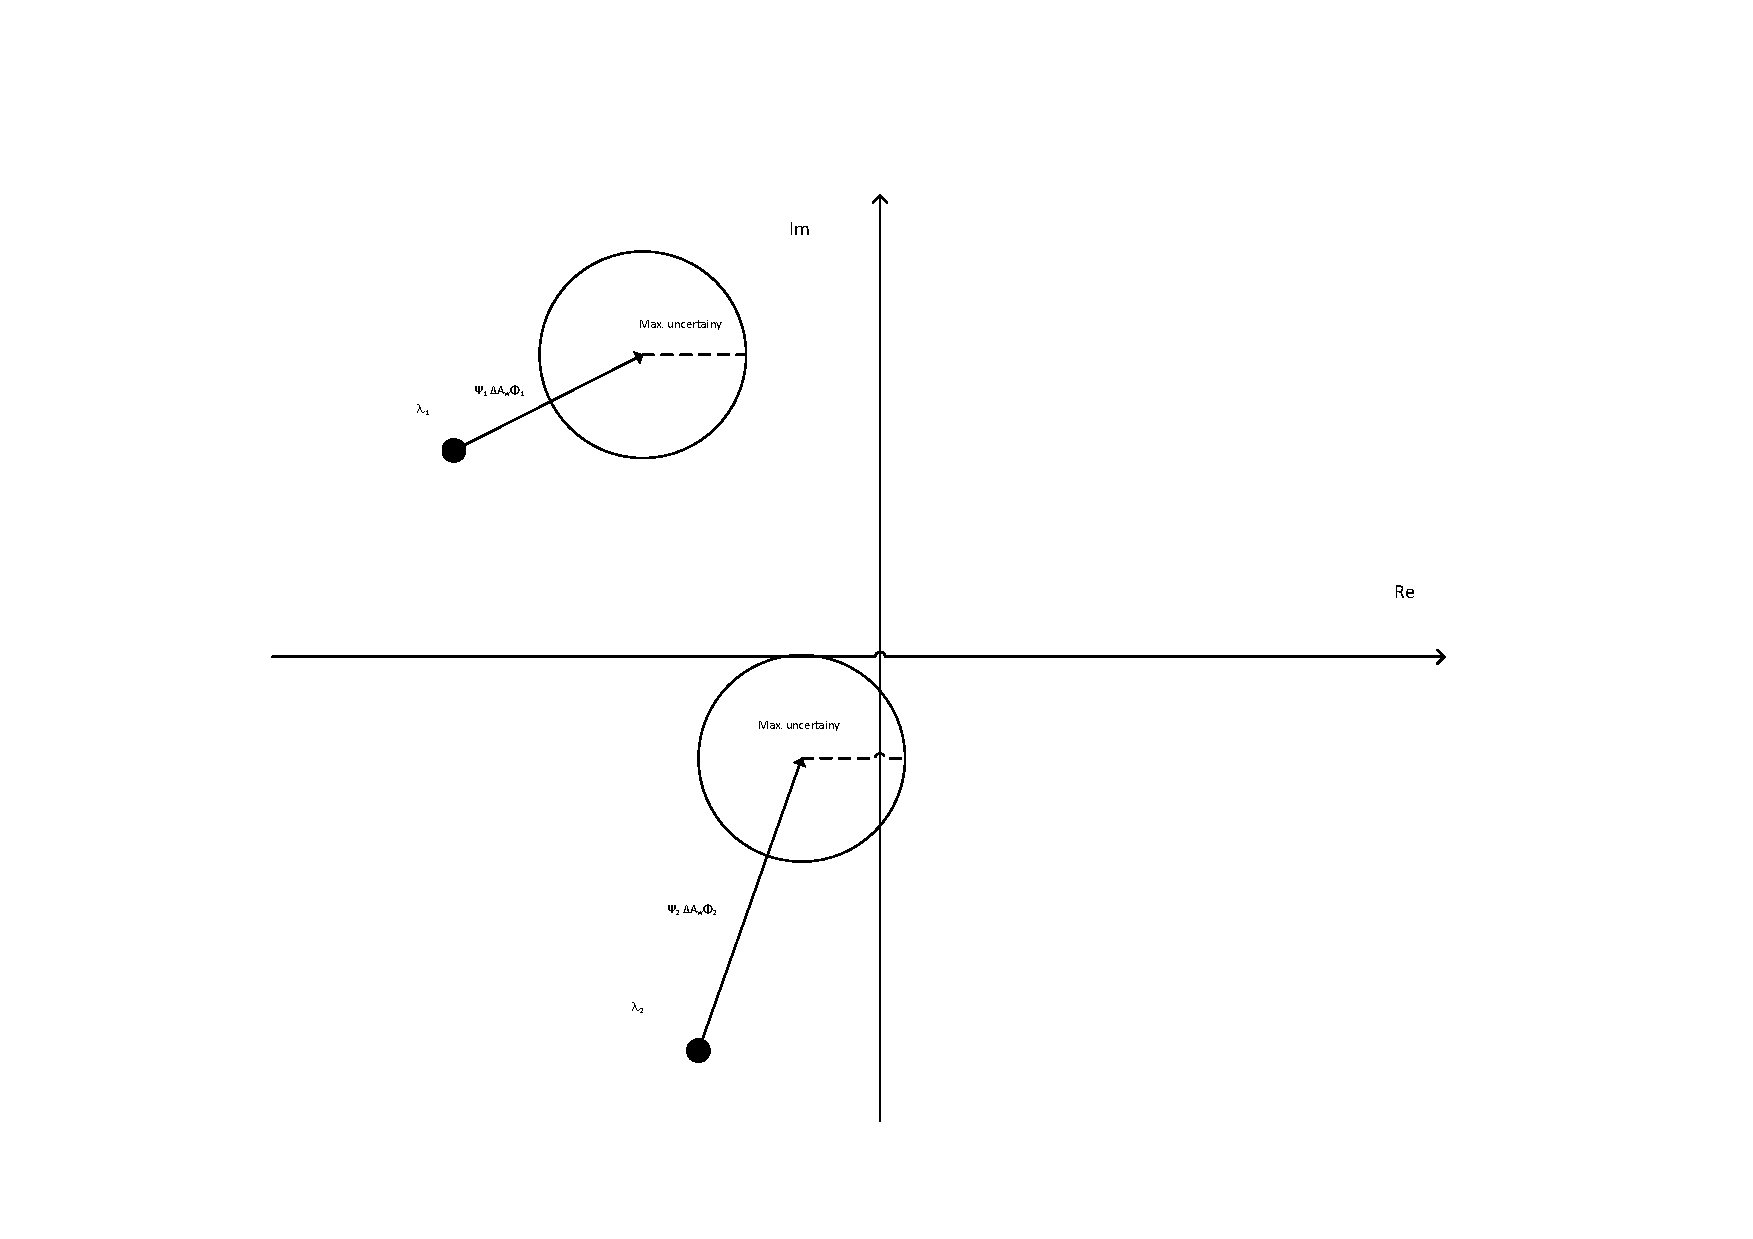
\includegraphics[width=\textwidth,height=\textheight,keepaspectratio]{Figures/Pole_changes.pdf}
 \caption{The estimate of $\lambda_1$ is somewhat stable, while there is a certain risk for $\lambda_2$ to become unstable}
 \label{fig:figure_of_the_method}
\end{figure}{}


\section{Guarantees of the estimate}
\label{sec:guarantees_of_estimate}
The difference between a real exponential and a Taylor-estimate is very dependant on if the exponent is larger than 0 or not. Just as a simple example, the two figures \cref{fig:fast_taylor} and \cref{fig:slow_taylor} shows how the difference between a Taylor-estimate and the real series develops with the number of steps in the Taylor-approximation. The sampling-rate should usually be fast enough to not be affected by the fastest dynamics, but it does not need to be true for stable dynamics. In practice, this might result in an algorithm that will give poor upper bounds for stiff systems. Since a circuit may contain very fast capacitors or indicators, a factor $e^{\norm{\Vec{A_s} T_s}}$ that becomes $e^100$ might be unlikely, but not that unreasonable. As seen from the graph, the result of such a matrix is that roughly 60 terms are needed to get rid of the most dramatic uncertainties. 
\begin{figure}
 \centering
 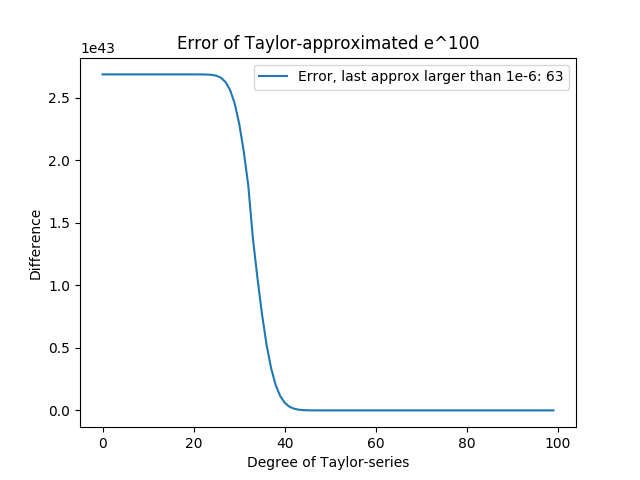
\includegraphics[width=\textwidth,height=\textheight,keepaspectratio]{Figures/taylor_estimate.png}
 \caption{Difference between real value and Taylor-estimate for $e^100$}
 \label{fig:fast_taylor}
\end{figure}{}

\begin{figure}
 \centering
 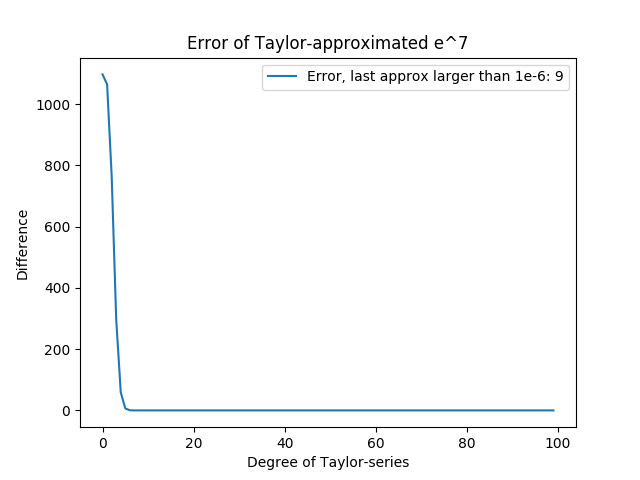
\includegraphics[width=\textwidth,height=\textheight,keepaspectratio]{Figures/taylor_estimate_slow_dyynamics.png}
 \caption{Difference between real value and Taylor-estimate for $e^3$}
 \label{fig:slow_taylor}
\end{figure}{}

\noindent
The true value of the estimates given by figures like \cref{fig:fast_taylor} and \cref{fig:slow_taylor} is that both the norm of $\Vec{A_s}$ and the norm of the derivative can be calculated before any more expensive computations are made. As can be seen from the plots, the Taylor-series has a certain number of steps that has to be exceeded before the precision starts increasing quickly. As a result, it is possible to say something about the number of steps in the Taylor-series that are needed to get a decent estimate. It even makes it possible to tell if the analysis will be worth it before any expensive computations have to be made. 

\section{Properties of electrical grids}

In the project, a lot of work had to be done in order to handle eigenvalues that are equal to zero. All RLC-circuits are passive systems, which in the case of linear systems also means that they are stable. As a result, there are cases where it might be reasonable to assume that no eigenvalues are equal to 0. Even when the system is not passive. There are still some issues with almost singular systems. The inverse of a system that is almost singular has always at least one eigenvalue that goes towards infinity. As a result, the norm of such a system will be very large and may be difficult to handle, since it will affect the norm of the inverted matrix quite severely. Depending on how quickly Taylor-series tend towards 0, the problem with ill-conditioned matrices might be a large one, or not bad at all. More testing with Taylor-series is most likely required. 
\noindent
The methods developed are also highly dependant on the type of problem that it is used on. In this project, it was assumed that it was very important that the system would not become unstable. Even more so than what is usually required in stability-analysis. This was done at the cost of scalability and ease of use. It is quite possible that, if other properties, like the non-linearities of a problem play a larger role than the time-delay, other methods will be much more useful. Finally, since all controller-parameters are described directly in the z-domain, it is much easier to analyze their effects on the w-domain. 



\chapter{Conclusion and future work}
\label{chp:conclusion}

\section{Conclusion} %# TODO The conclusion must be finished soon
Analysing discretised systems in the z-domain tends to be a difficult task, and the results provided in this project did not change that. The method that was provided here did, however provide a tool that should, at least, in theory give estimates that will be pessimistic. That is something that can be useful for problems, where the cost of failure is very large. Furthermore, the uncertainties of the estimates come from the limited ability to perform matrix-multiplications. That means, that as computational power increases, it will be possible to analyse larger systems, or with less error. During the project, no methods were found that could provide a general solution, which will work on any linear system. In return, the solution that was provided covers a wide class of linear systems, and will be valid for most physical systems, and all passive ones. There was not enough time in the project to implement the algorithm, and test for how tight the bounds for the estimates would have been. From the rough estimate of the bounds in \cref{sec:guarantees_of_estimate}, the current upper bound may work very poorly for stiff systems, since calculating the derivative of a Taylor-series with 60 steps is unreasonable for a matrix in $\Re^{1000\times 1000}$


\todo[inline]{I left off here}
\section{Future work}
Since there was not enough time to test the method that was developed in this project, the most important task forward will be to simulate the methods provided, and see if they work in practice.

\noindent
As a secondary goal, it is also relevant to see if the upper bounds that were given on the derivatives are tight enough to be used. It is deffinitely possible that tighter bounds can be given. Differentiating the Taylor-approximations grows more or less cubically with the number of steps done in the Taylor-approximating. Additionally, the norm given by the matrices will grow with the number of elements, so the method may scale poorly. So tighter bounds might also be needed. 

\noindent
It is potentially of equal importantance to try to describe inputs properly in the w-domain. This project was only able to say something about modeling errors, and not anything about noise. It is possible that if it would be possible express inputs in the w-domain, something valueble could be said about the robustness to noise. 

Furthermore, the method is not general, so there may be ways to always give an upper bound on the derivative, even for singular system-matrices where the eigenvalues are 0, and change depending on the parameters. After asking some people who work in the field of mathematics to take a quick glance at the problem, they mentioned that the problem looked close to something that could be solved with a pseudo-inverse. The awnsers were mostly based on a huch, but it may be worth looking into. It has also been mentioned that Higham's Complex Step Approximation is a good estimator for $\frac{d e^{\Vec{A}(\rho)}}{d \rho }$, but there was not enough time to explore it further, or to see if it was possible to give any guarantees with regards to the error. 

\noindent

Additionally, a lot of work remains on the practical side. The model explored in this paper is one of the simplest set-ups for a \gls{VSC}, and does not cover concepts such as multiple controllers on a grid, variable sources, or different kinds of controllers. 


\appendix

\chapter{ Appendix }
\label{chp:appendix}
\section{Pulse-Width Modulator PWM}
\label{sec:PWM}

\todo[inline]{A short explanation of a PWM, or referencing a source/learning-material}
When attempting to go from a discrete signal from a controller to a continuous electrical voltage, one of the most common ways of doing that is by using Pulse-width modulation. 
\begin{figure}
    \centering
    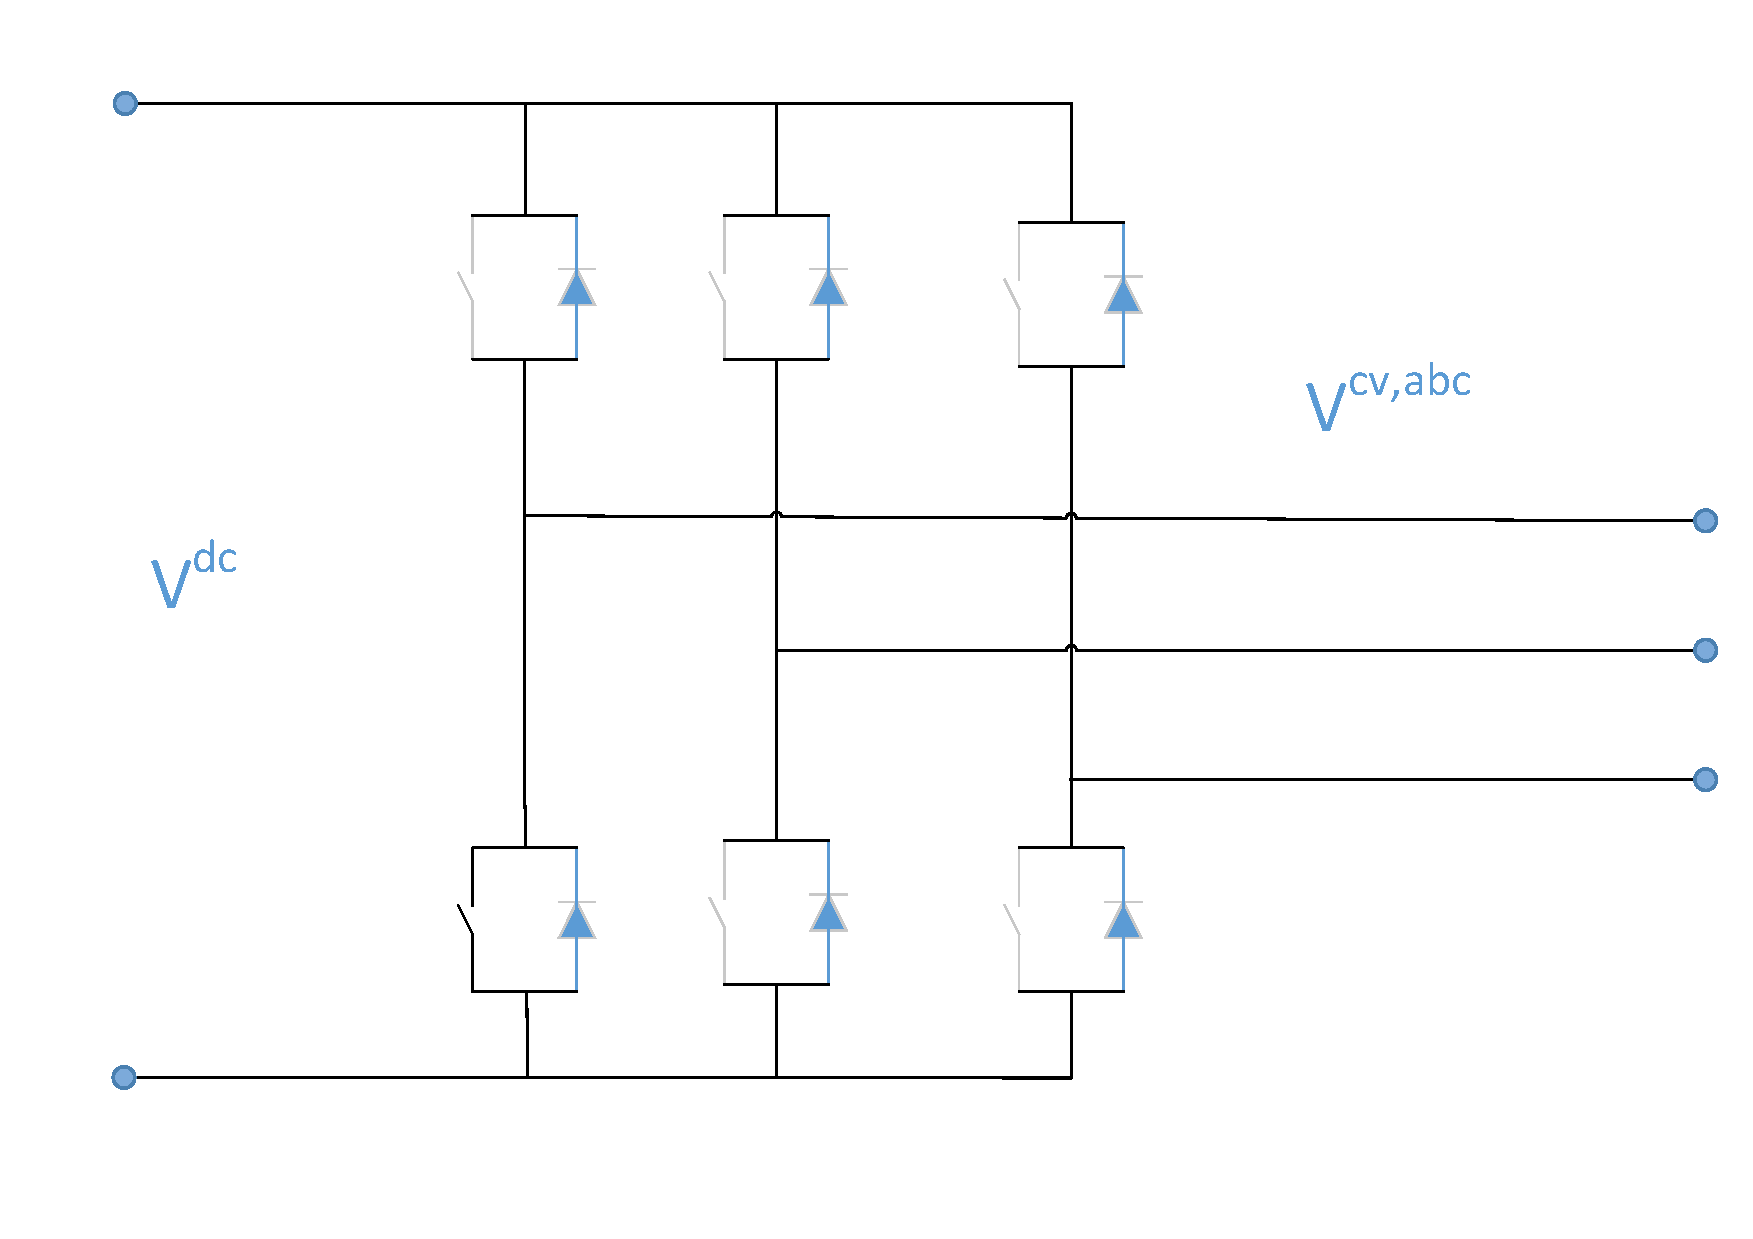
\includegraphics[width=\textwidth,height=\textheight,keepaspectratio]{Figures/Inverter.pdf}
    \caption{An inverter without the necessary filters on the AC or DC-side, (Inspired by \cite{Suul_electro_presentation_1})}
    \label{fig:PWM}
\end{figure}{}
In order to make different voltages on a line, a \gls{PWM} can only keep a connect a voltage to a high or a low voltage. The operates on short periods, where a certain fraction of that period is spent with a line connected to the high voltage, and the rest of the time, connected to the low one. This results in a voltage that jumps between two extremes at least once per period. In order to make a sine-wave the sluggishness of a RLC-circuit is used to make the voltage appear somewhat more smooth, and follow something that resembles more what the desired voltage should be. 

\begin{figure}
    \centering
    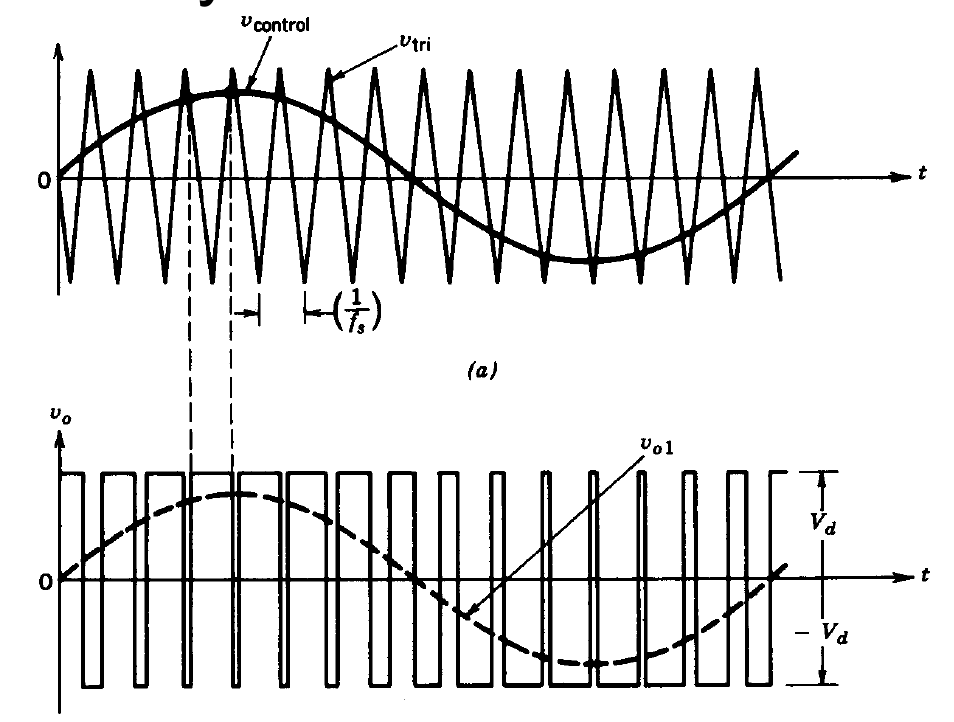
\includegraphics[width=\textwidth,height=\textheight,keepaspectratio]{Figures/PWM_response.png}
    \caption{Output-voltage from \gls{VSC}, given voltage reference and a low-pass filter \cite{Suul_electro_presentation_1}}
    \label{fig:PWM_response}
\end{figure}{}

The reference is usually in periodic intervals, and is given by the duty-cycle. The duty cycle is how long the voltage is high over a period. For a gate to be high, the upper gate of the inverter has to be open, while the lower one has to be closed. And it is the opposite to get a low voltage. 


\section{Park- and Clarke transformation and rotating reference frames}
\label{sec:rotating_reference_frame}
A normal three-phase AC current usually follows three sinusoidal waves that have a \ang{120} phase difference between each other. 

\begin{equation}
\begin{aligned}
    \label{eq:three_phase}
        V_a &= \hat{V}_a \cdot \sin{(\omega t + \phi )}\\
        V_b &= \hat{V}_b \cdot \sin{(\omega t + \phi + \frac{2\pi}{3} )}\\
        V_c &= \hat{V}_c \cdot \sin{(\omega t + \phi - \frac{2\pi}{3} )}
    \end{aligned}
\end{equation}
\begin{equation}
    V_{abc} = 
    \begin{pmatrix}
        V_a \\ 
        V_b \\ 
        V_c
    \end{pmatrix}
\end{equation}{}
If the system is balanced, the three voltages will always add up to 0. This means that we have a three-dimensional representation of the electrical lines, where one dimension is redundant. We can reduce the number of dimensions in a three-phased system by performing the Clarke-transformations, which rotates the reference-frame in such a way that one of the axis represents a scaled sum  of all three phases.  \cite{Clarke_transform_source}. Deriving the rotation-matrix is somewhat difficult, but the resulting rotation matrix will represent the Clarke-transformation from the $abc$ frame to the $\alpha\beta 0$ frame. 


\begin{equation}{}
    \label{eq:Clarke_transform}
    V_{\alpha\beta 0} = \frac{2}{3}
    \cdot
    \begin{bmatrix}
        1                   & -\frac{1}{2}          & -\frac{1}{2} \\
        0                   & \frac{\sqrt{3}}{2}    & -\frac{\sqrt{3}}{2} \\
        \frac{1}{\sqrt{2}}  & \frac{1}{\sqrt{2}}    & \frac{1}{\sqrt{2}}
    \end{bmatrix}
    V_{abc}
\end{equation}{}


\begin{figure}
    \centering
    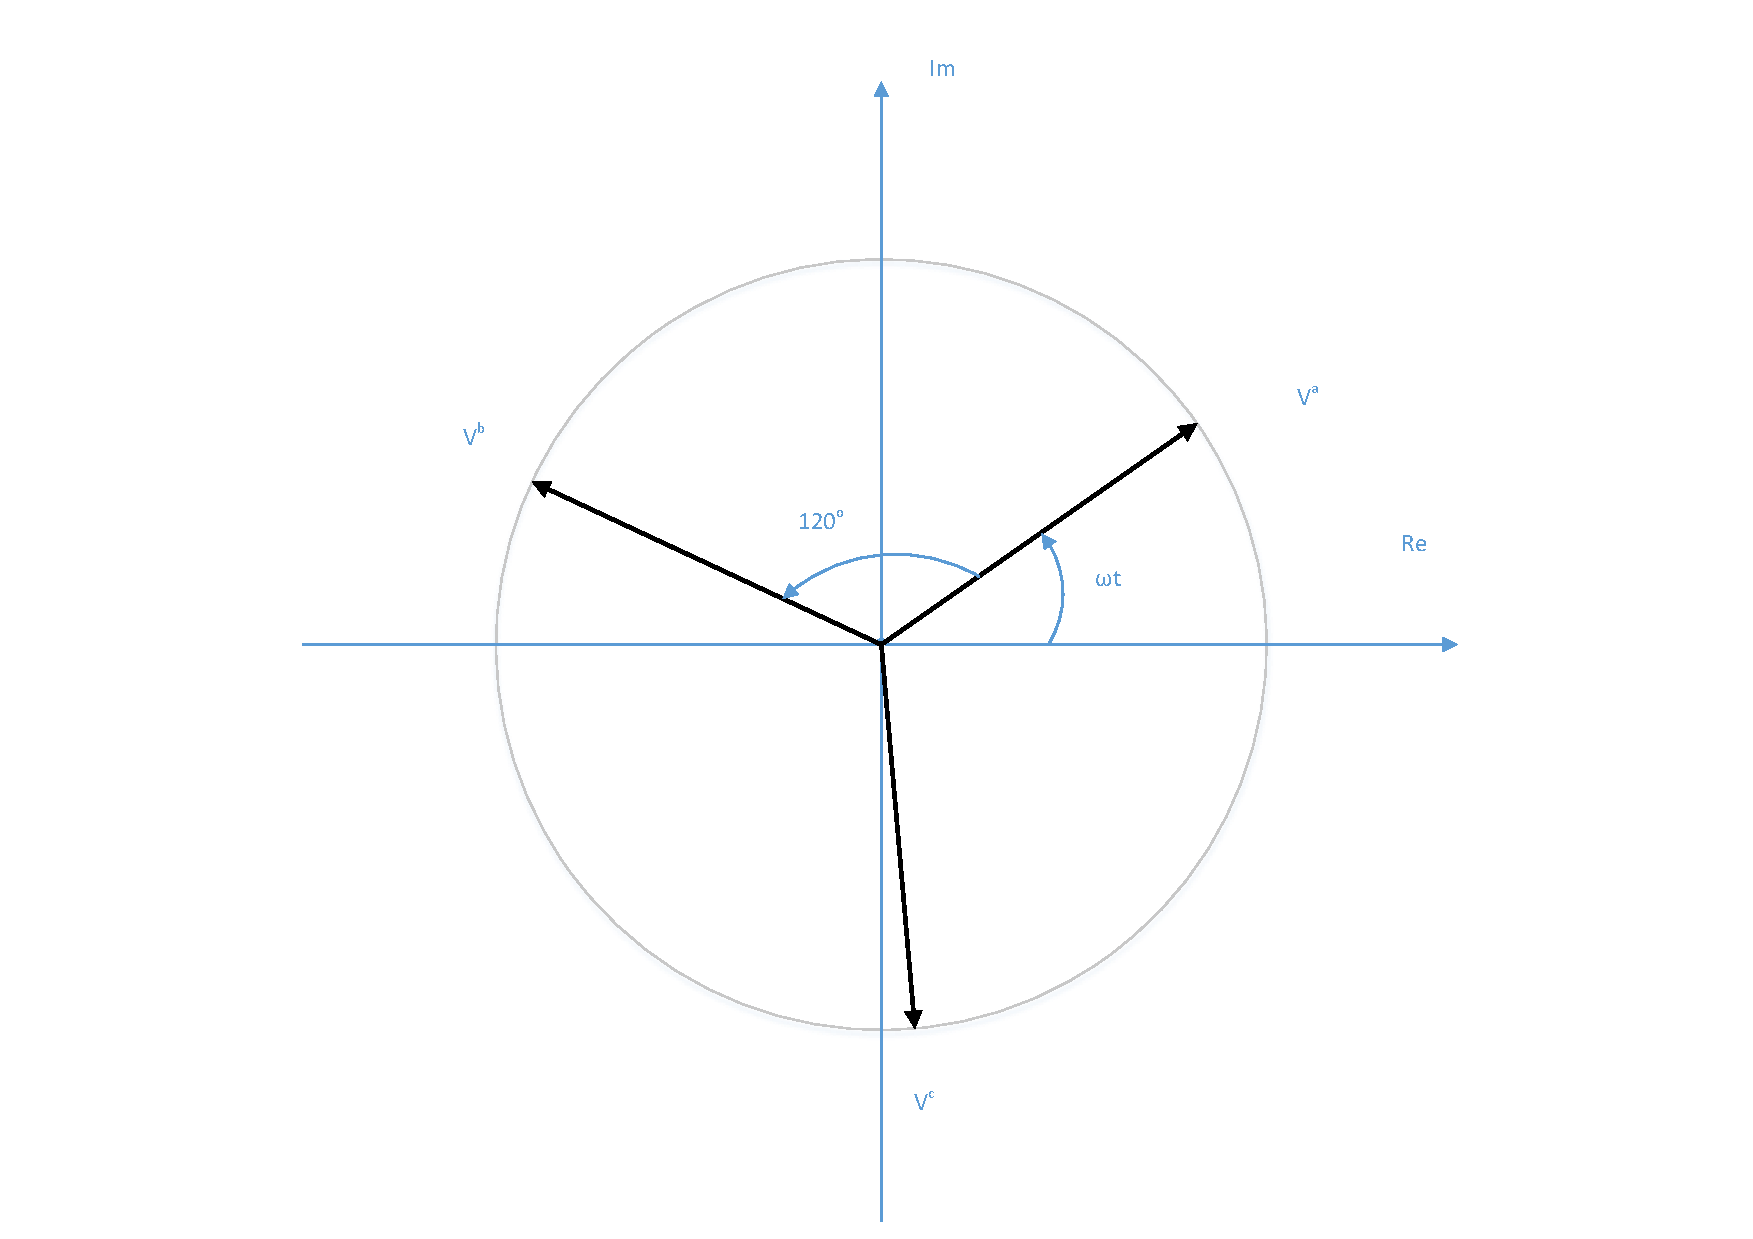
\includegraphics[width=\textwidth,height=\textheight,keepaspectratio]{Figures/Untransformed_phase.pdf}
    \caption{A representation of the three-phase system in the complex plane, when following the abc-reference frame}
    \label{fig:Current_circle}
\end{figure}


The Park transformation consists of rotating the $\alpha$ and $\beta$ axes by some arbitrary frequency. something within this reference frame has the same angular velocity as the rotation, it will be perceived  as a DC-current in the dq0- reference frame.  When looking at the transformation in  \Cref{fig:Current_circle}, it can be seen that if all components of the three-phase voltage are represented as orthogonal complex numbers along some circle.




\begin{figure}
    \centering
    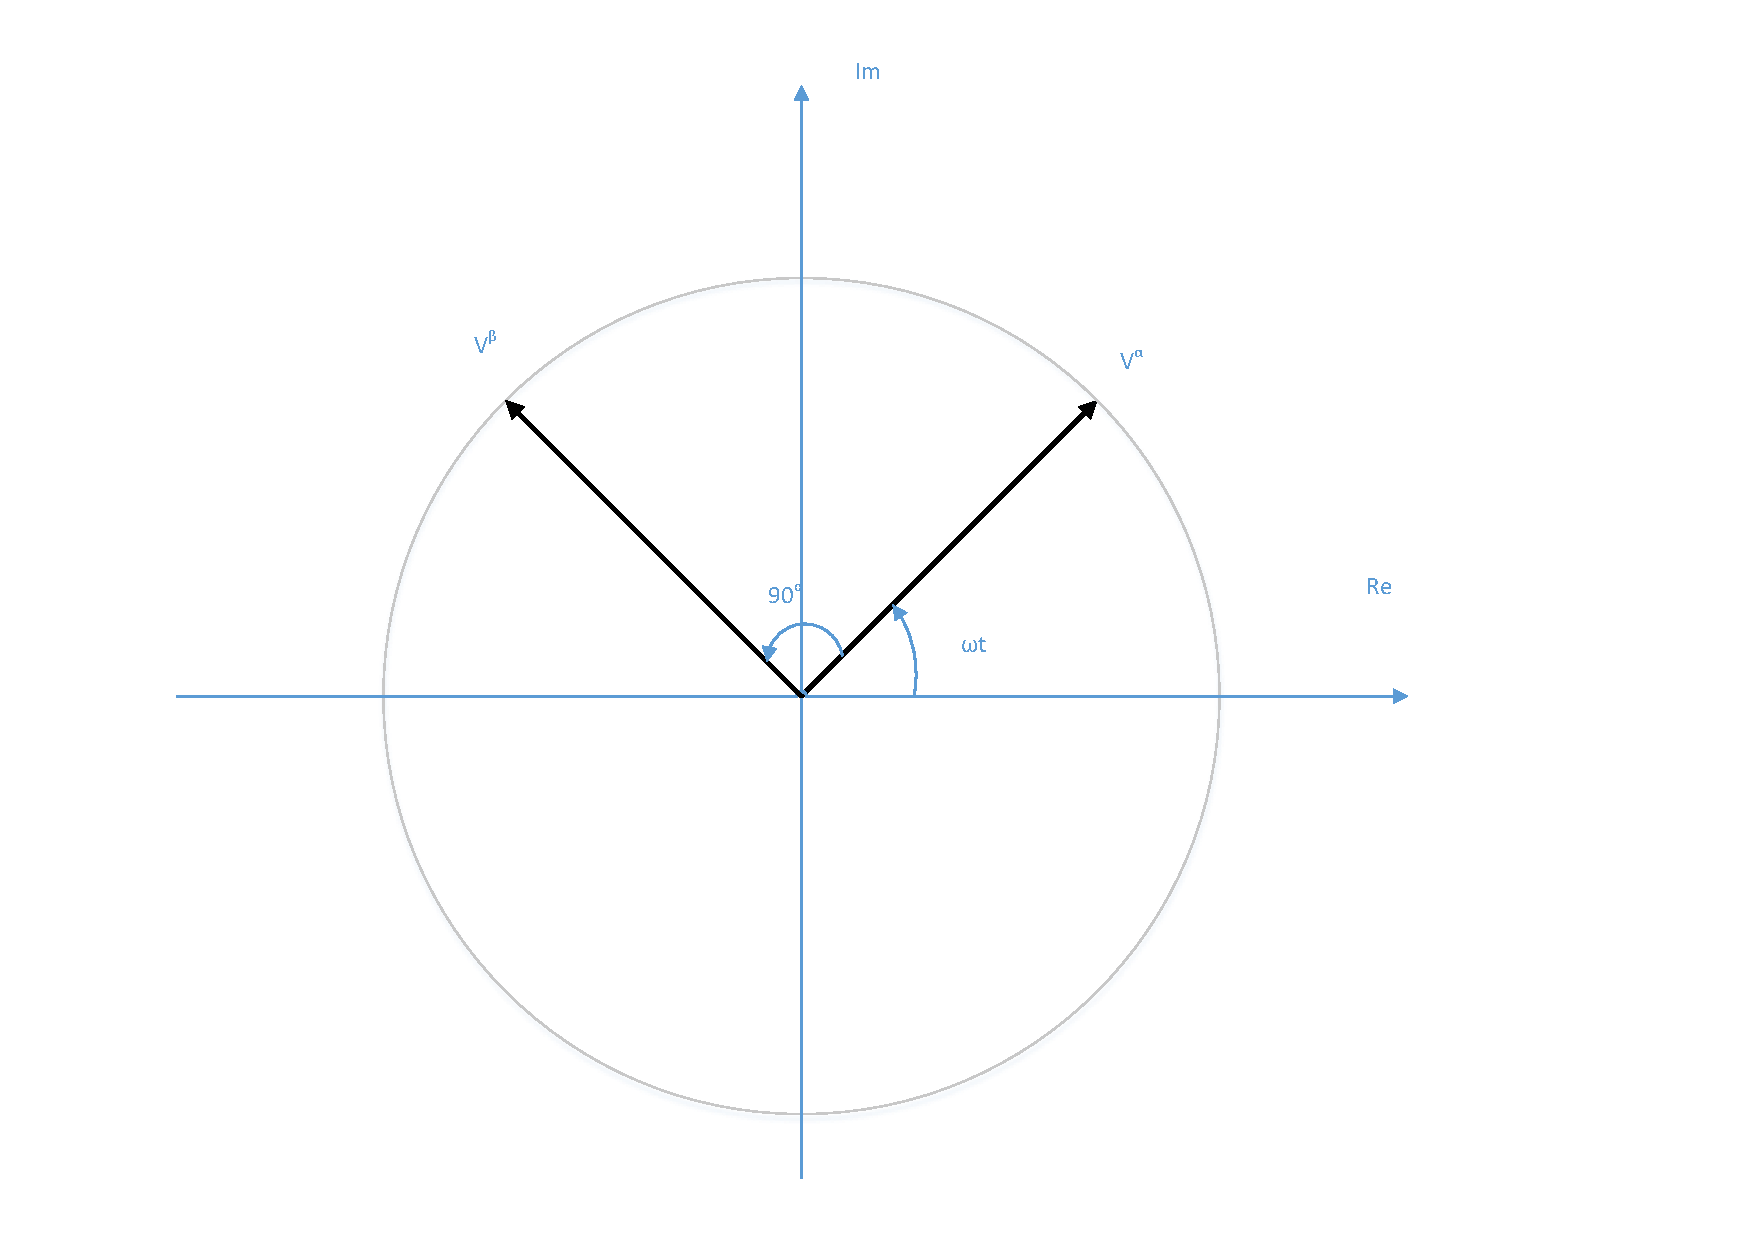
\includegraphics[width=\textwidth,height=\textheight,keepaspectratio]{Figures/Clarke_transformed.pdf}
    \caption{$\alpha$ and $\beta$ after the Clarke transformation. The phases are rotating $90^{\circ}$ from each other}
    \label{fig:First_clarke_transformation}
\end{figure}

\begin{figure}
    \centering
    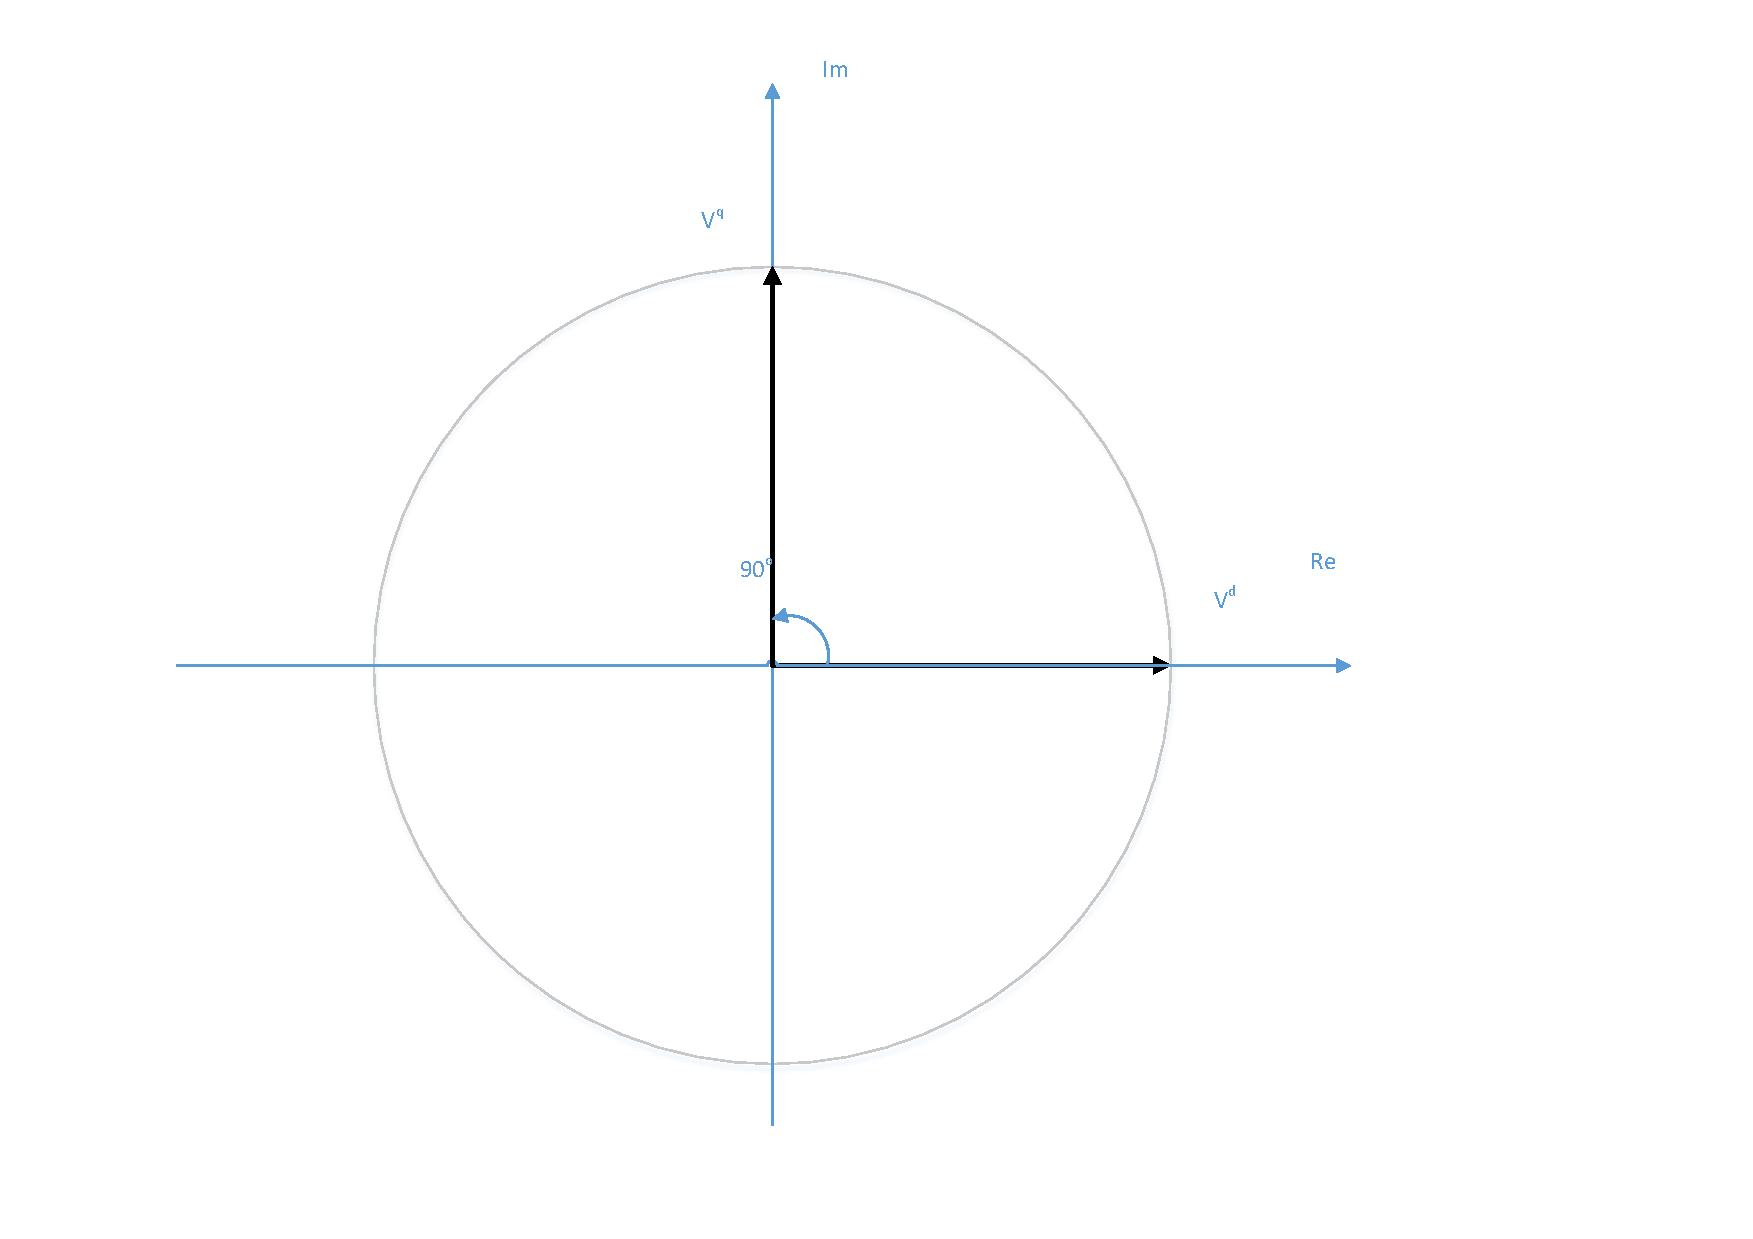
\includegraphics[width=\textwidth,height=\textheight,keepaspectratio]{Figures/Park_transformed.pdf}
    \caption{$d$ and $q$ after the Park transformation. The current-vectors no longer rotate in the complex plane if they had the same angular frequency as the transformation}
    \label{fig:Park_transformed}
\end{figure}

The vectors for abc, can be seen as rotating with an angular velocity $\omega$ as time passes, and if the value along the $\alpha$-axis is seen as the real value, while the value along the $\beta$ axis is seen as the imaginary one, the rotation 
\begin{equation}
    R_{park} = \begin{bmatrix}
       \cos{\left(\theta\right)} & \sin{\left(\theta\right)} \\
       -\sin{\left(\theta\right)} & \cos{\left(\theta\right)}\\

    \end{bmatrix}
\end{equation}

can be seen as a multiplication with $e^{-j\theta}$. Thus, if theta is the same as $\omega t$, the angle of $V_{dq} = R_{park}V_{\alpha\beta}$ will always remain constant, and the ac-voltage is observed as a DC-voltage. 

The Clarke, and the Park transformation can be combined into the DQZ-transformation. 

\begin{equation}
 \sqrt{\frac{2}{3}}\begin{bmatrix}
   \cos{\left(\theta\right)}
      & \cos{\left(\theta - \frac{2\pi}{3}\right)}
      & \cos{\left(\theta + \frac{2\pi}{3}\right)} \\
   -\sin{\left(\theta\right)}
      & -\sin{\left(\theta - \frac{2\pi}{3}\right)}
      & -\sin{\left(\theta + \frac{2\pi}{3}\right)} \\
   \frac{\sqrt{2}}{2}
      & \frac{\sqrt{2}}{2}
      & \frac{\sqrt{2}}{2}
\end{bmatrix}
\end{equation}{}


The dq0- transformation is a non-linear transformation that makes it possible to observe the frequency and the amplitude of an AC-voltage of one specific frequency as something constant. This makes it possible view the system as a time-invariant one. This is a necessary condition if a normal PI-regulator is supposed to be able to control the system towards zero deviation from the reference. 


    
\section{Exact response from a Polynomial input }    
\todo[inline]{Bedre tittel på denne delen}
\label{sec:finding_response_from_polynomial_inputs}
$e^{\Vec{A}t}$ is defines as 
\begin{equation}
    e^{\Vec{A}t} \triangleq  \sum_{n=0}^\infty A^n \frac{t^n}{n!}
\end{equation}{}
To show that the time-response for any $\Vec{x}(t)$, as long as $\Vec{u}(t)$ is constant, we approximate $\Vec{x}(t)$ by a Taylor series. 
\begin{equation}
    \dot{\Vec{x}} = \Vec{A}\Vec{x} + \Vec{Bu}
\end{equation}{}
    
\begin{equation}
    \ddot{\Vec{x}} = \frac{d}{dt} \left( \Vec{A}\Vec{x} + \Vec{Bu} \right) = \Vec{A}( \Vec{Ax}+ \Vec{Bu}) + \Vec{B \dot{u} }
\end{equation}{}

\begin{equation}
    \frac{d^n\Vec{x}}{dt^n} = \Vec{A}^nx + \sum_{m=1}^n \Vec{A}^{n-m}\Vec{B}\frac{d^{m-1}\Vec{u}}{dt^{m-1}}
\end{equation}{}

\begin{figure}
    \centering
    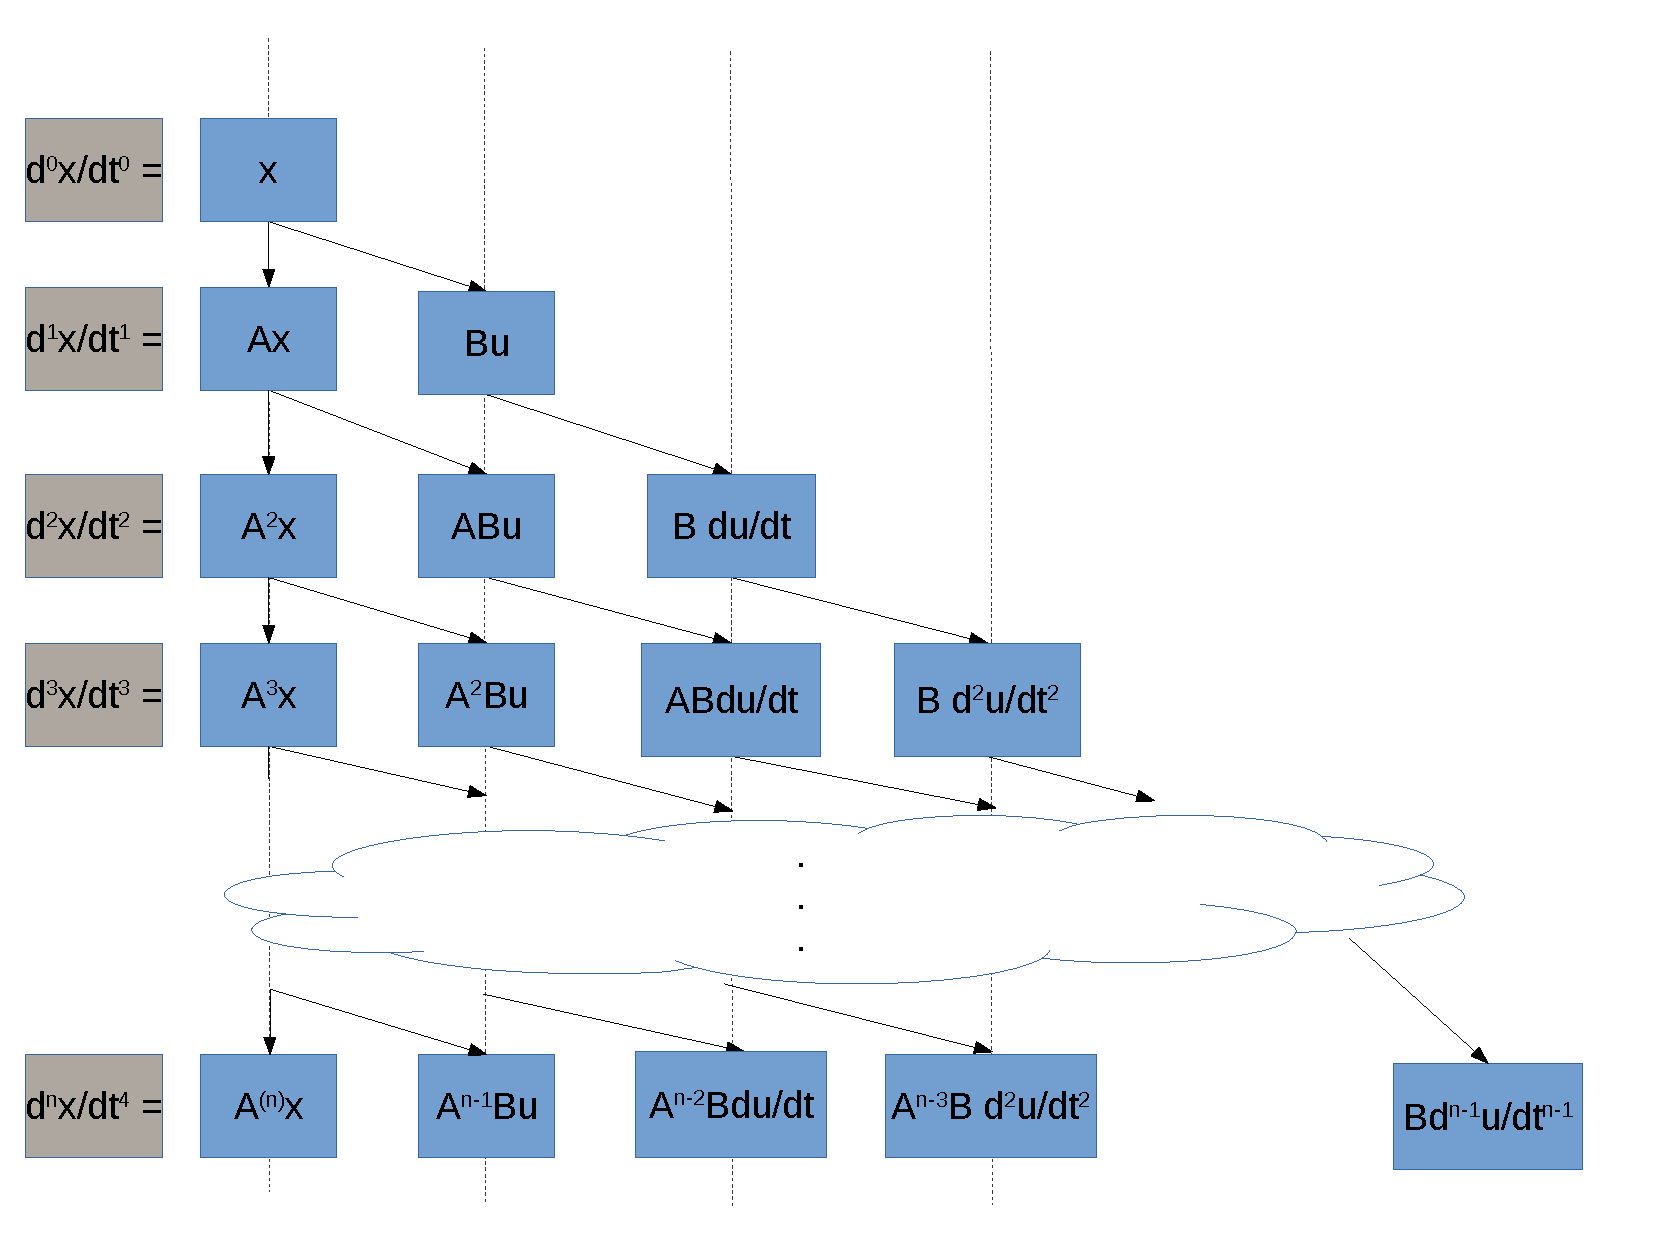
\includegraphics[width=\textwidth,height=\textheight,keepaspectratio]{Figures/Derivasjons_figur.pdf}
    \caption{Structure of the nth derivative of x}
    \label{fig:derivative_figure}
\end{figure}
Which has the same structure as \cref{fig:derivative_figure}

If $\Vec{u}$ has a finite number of derivatives, it will be possible to use the Taylor-series of $e^{\Vec{A}t}$ to give the exact series that are proportional to any derivative of $\Vec{u}$. Each step from $n > m$ in the sequence can be expressed as 
\begin{equation}
    \Vec{A}^{n-m}\Vec{B}\frac{d^{m-1}\Vec{u}}{dt^{m-1}}
\end{equation}{}

Which means, that if we can subtract the first m terms from $\Vec{A}^{-m-1}e^{\Vec{A}t}$, it is possible to express $\Vec{x}(t)$ as 

\begin{equation}
    \Vec{x}(t) = e^{\Vec{A}t}\Vec{x(0)} + \sum_{m=0}^M A^{-m-1}\left( e^{\Vec{A}t}\Vec{x(0)} - \sum_{i=0}^{m}\frac{\Vec{A}^i}{i!} \right)\Vec{B}\frac{d^m\Vec{u}}{dt^m}(0)
\end{equation}{}
where $M$ is the highest order derivative of $\Vec{u}$. This means that it is possible to get an exact solution of a linear system for any input u, that can be expressed as a finite polynomial. 

If the time-step $t=T_s$ is known in advance, it is possible to make a matrix $e^{\Vec{A}T_s}$ in advance, which can give an exact solution for any initial state. The response from the inputs will have to be a sum of products different matrices and the derivatives of $\Vec{u}$, where each matrix is constant, possibly different for each derivative.


But whenever somebody solves linear systems, $M$ is almost always equal to 1, which gives the simpler equation. 

\begin{equation}
        \Vec{x}(t) = e^{\Vec{A}t}\Vec{x(0)} + \Vec{A}^{-1}\left( e^{\Vec{A}t}\Vec{x(0)} - \Vec{I} \right)\Vec{u}
\end{equation}{}

But, we will sadly need the general solution for if the system matrix has Jordan-blocks with eigenvalues equal to 0, that are larger than $(1x1)$

\todo[inline]{Gjør denne litt mer presis}
    



\section{Finding \texorpdfstring{$e^{\Vec{A}t}$}{}  when A is  defective}
\label{sec:finding_eAt_when_A_is_defective}
Normally, when trying to find the exact solution of a linear system, given some initial values, it is done by diagonalising the matrix $\Vec{A}$, and then solving the much simpler set of first order equations that don't interact with each other. But, not all matrices are diagonalisable. One such example is: 
\begin{equation}
    A_{deg} = 
    \begin{bmatrix}
        0 & 1 \\ 
        0 & 0 
    \end{bmatrix}
\end{equation}
Luckily, all matrices can be written on Jordan-form \cite[Chp 1]{Triangle_inequality_source}, where each vector in the basis satisfies. 
\begin{equation}
    (\Vec{A}- \lambda_i \Vec{I})\Vec{e_i} = 0
\end{equation}
or
\begin{equation}
    \exists e_j s.t  (\Vec{A}- \lambda_i \Vec{I})\Vec{e_i} = \Vec{e_j}
\end{equation}
In these cases, the matrix $\Vec{A}$ can be written on a form $\Vec{Q^{-1} J Q}$. where $\Vec{J}$ is a block-diagonal matrix, where each block has a diagonal corresponding to an eigenvalue, and a superdiagonal with elements equal to 1. As a result, each Jordan-block can be solved separately. 
\begin{equation}
    \Vec{J_i} = 
    \begin{bmatrix}
        \lambda_i & 1         & 0      & \cdots &0          &0\\
        0         & \lambda_i & 1      &\cdots  & 0         &0\\
        \vdots    & \vdots    & \ddots & \ddots & \vdots    & \vdots \\
        \vdots    & \vdots    & \ddots & \ddots & \vdots    & \vdots \\
        0         & 0         & 0      & \cdots & \lambda_i & 1 \\
        0         & 0         & 0      & \cdots & 0         & \lambda_i \\
    \end{bmatrix}
\end{equation}

Each Jordan-block can be solved by first solving the independent equation, and working upwards from there. Take note that we will break notation and refer to the lowest state in the Jordan-block as $q_1$ and work our way upwards to $q_n$. 
\begin{equation}
    q_1 = \lambda_i q_1 
\end{equation}
Which gives an expression $q_1(t)= q_1(0) e^{\lambda_i t}$. The following element will be the solution of 
\begin{equation}
    q_2 = \lambda_i q_2 + e^{\lambda_i t}q_1(0)
\end{equation}
Which can be solved by $q_2(t)  = e^{\lambda_i t}q_2(0) + t e^{\lambda_i t}q_i(0)$. As we can see, a pattern emerges quickly, where the product-rule together with an an exponential is used to describe both a state $q_i$ and its predecessor $q_{i+1}$. But, since the derivative of $t^n = nt^{n-1}$, a the result will also have to be multiplied by a constant. The result is something along the lines of: 
\begin{equation}
    q_{j}(t) = q_j(0)e^{\lambda_i t} + \sum_{k=1}^n \frac{t^{k}}{k!}q_{j-k}(0)e^{\lambda_i t} 
\end{equation}
The resulting matrix for the solution becomes. 
\begin{equation}
    e^{\Vec{J_i} t } = e^{\lambda_i t} 
    \begin{bmatrix}
        1      & \frac{t}{1!} & \frac{t^2}{2!} & \frac{t^3}{3!} &\cdots  & \frac{t^{n-1}}{(n-1)!} & \frac{t^n}{n!}\\
        0      & 1            & \frac{t}{1!}   &\frac{t^2}{2!}  & \cdots & \frac{t^{n-2}}{(n-2)!} & \frac{t^{n-1}}{(n-1)!}\\
        0      & 0            & 1              & t              & \cdots & \frac{t^{n-3}}{(n-3)!} & \frac{t^{n-2}}{(n-2)!} \\
        \vdots & \vdots       & \vdots         &\vdots          & \ddots & \vdots                   & \vdots \\
        0      & 0            & 0              & 0              & \cdots & 1                        & \frac{t}{1!} \\
        0      & 0            & 0              &0               & \cdots & 0                        & 1
    \end{bmatrix}
\end{equation}
This also means that $e^{\Vec{J_i} t }$ is a solution of the Taylor-series including $\Vec{J}$. And since $\Vec{A}= \Vec{Q^{-1}JQ}$, the Taylor-series of A will mostly contain cancellations between $\Vec{Q}$ and $\Vec{Q}^{-1}$, making each term into $\Vec{\frac{t^n}{n!} Q^{-1}J^nQ}$. This means that the solution for $e^{\Vec{J}t}$
\begin{equation}
    e^{\Vec{A}t} = \Vec{Q}^{-1}e^{\Vec{J_i} t }\Vec{Q} 
\end{equation}

As a result, it is possible to find the exact response for a linear system. Even if the number of eigenvectors is too small to cover the entire space. 



\section{Finding exact step-response when A is non-invertible}
\label{sec:solving_for_uninvertible_matrices}
When finding the system-response for constant input, it is usually found by using the expression
\begin{equation}
    \Vec{A}^{-1} \left( e^{\Vec{A}t} - \Vec{I}\right)
\end{equation}
But if $\Vec{A}$ has any eigenvectors that are equal to 0, then $\Vec{A}$ will not be invertible. As a result, this method will not work directly. On the other hand, from the analysis in \cref{sec:finding_response_from_polynomial_inputs}, we saw that the input-response is still given by a Taylor-series, so it definitely exists. 
If the system is written on Jordan canonical form the problem is solvable. We can invert  and solve normally for any block where $\lambda_i \neq 0$. In the case of the subspace where $\lambda_i =0$, set it the non-existent inverted Jordan-block to be 0, so that it can be solved later. We call this pseudo-inverted matrix $J^{-1}_{pi}$.
The interesting parts about Jordan-blocks when the eigenvalues are 0 is that each state will act as a pure integrator with respect to something. As a result, the input-response for the sub-space will act very similarly to the impulse response for a system with eigenvalues equal to 0. The only difference is that the first (constant) state is replaced by a constant input instead. 

Therefore, if the Jordan-block looks like this 

\begin{equation}
    \begin{bmatrix}{}
    \lambda_i & 1 & 0 &\dots &\dots & 0 & 0  \\
    0 & \lambda_i & 1 & \dots &\dots & 0 & 0 \\
    \vdots & \vdots & \vdots & \ddots & \ddots & \vdots & \vdots &\\
    \vdots & \vdots & \vdots & \ddots & \ddots & \vdots & \vdots &\\
    0 & 0 & 0 & \dots  & \dots & \lambda_i & 1 \\ 
    0 & 0 & 0  & \dots & \dots & 0 & \lambda_i \\
    \end{bmatrix}
\end{equation}{}

and $\lambda_i =0$, the exact solution will look like: \\

\begin{equation}
    \gls{step_resp}_{\lambda=0}(t) = 
\begin{bmatrix}{}

t & \frac{t^2}{2!} & \frac{t^3}{3!} &\dots &\dots & 0 & \frac{t^n}{n!} \\
 0 & t & \frac{t^2}{2!} & \dots &\dots & 0 & \frac{t^{n-1}}{(n-1)!} \\
 
 \vdots & \vdots & \vdots & \ddots & \ddots & \vdots & \vdots\\
 
 \vdots & \vdots & \vdots & \ddots & \ddots & \vdots & \vdots\\
 
 0 & 0 & 0 & \dots & \dots & t & \frac{t^2}{2!} \\
 
 0 & 0 & 0 & \dots & \dots & 0 & t \\
\end{bmatrix}
\end{equation}{}
So if a specialised block-diagonal matrix $\gls{step_resp}_{non\_inv}$, where all values are 0, except for the block $\gls{step_resp}_{\lambda=0}(t)$ for the subspace that belongs to the singular Jordan-block. 


\begin{equation}
    \Vec{x}(t) = e^{\Vec{A}t}\Vec{x}(0) + \Vec{Q}^{-1}\Vec{J}^{-1}_{pi}\Vec{Q}(e^{\Vec{A}t}\Vec{x} - \Vec{I})\Vec{Bu} + \gls{step_resp}_{non\_inv}(t) \Vec{Bu}
\end{equation}{}

If the time-step is a known constant, then the two matrices from the input can be combined into one constant matrix. 



\section{Differentiating the step-response of a non-invertible system}
\label{sec:differentiating_step_response_from_input}
Normally
\begin{equation}
    \frac{d \gls{step_resp}}{d \rho} = \frac{d\Vec{A^{-1}}}{d \rho} \left( e^{\Vec{A}t} - \Vec{I}\right)\Vec{B} + \Vec{A}^{-1} \left( \frac{de^{\Vec{A}t}}{d\rho}\right)\Vec{B} +  \Vec{A^{-1}} \left( e^{\Vec{A}t} - \Vec{I}\right)\frac{d\Vec{B}}{d\rho}
\end{equation}
This solution is obviously not possible if A can't be inverted, so an alternative has to be found. In this project, no general solution was found for this problem. But, if the subspace, made out of generalised eigenvectors, with eigenvalues equal to 0 is unaffected by $\rho$, then it is possible perform a change of basis, by using a matrix $\Vec{Q}$

Which leads to 
\begin{equation}
    \Vec{Q}^{-1}\Vec{q} = \Vec{x}
\end{equation}
\begin{equation}
    \dot{\Vec{q}} = \Vec{QAQ}^{-1}\Vec{q} + \Vec{QB}\Vec{u}
\end{equation}

If $\Vec{Q}$ is chosen properly, it is possible to separate the system into a well-behaved part, and the part where the eigenvalues are equal to 0.
\begin{equation}
    \dot{\Vec{q}}=
    \begin{bmatrix}
        \Vec{A}_{sub} & \Vec{A}_{1,2}\\
        \Vec{0} & \Vec{J}_{\lambda=0}
    \end{bmatrix}
    \Vec{q}
    + 
    \begin{bmatrix}
        \Vec{B}_{sub}\\
        \Vec{B}_{\lambda=0}
    \end{bmatrix}
    \Vec{u}
\end{equation}
Because of this separation, $\Vec{q}$ can be split into two parts
\begin{equation}
    \Vec{q}= \begin{bmatrix}
        \Vec{q_{sub}}\\
        \Vec{q}_{\lambda =0}
    \end{bmatrix}
\end{equation}
\todo[inline]{Bedre navn på koblingen mellom dem}


One transformation that can split the system into two parts, like this is the transformation into Jordan-canonical form. But, in order to make the differentiation simpler, the same transform is used, even after $\rho$ might have changed the bases of $\Vec{A}_{sub}$. This makes the differentiation a lot easier. 
\noindent
If $\Vec{B}_{\lambda=0}$ is unaffected by $\rho$, then $\Vec{q}_{\lambda=0}$ can be solved independently. Each Jordan-block will have a solution on the form: 
\begin{equation}
    \gls{step_resp}_{Jordan\_block} = 
    \begin{bmatrix}
        t & \frac{t^2}{2!} & \cdots & \frac{t^{n}}{n}\\
        0 & t  & \cdots & \frac{t^{n-1}}{(n-1)!}\\
        \vdots & \vdots & \ddots & \vdots & \\
        0 & 0 & \cdots & t
    \end{bmatrix}    
\end{equation}
Where n is the number of linearly independent generalised eigenvectors that result from an ordinary eigenvector (including itself). As a result, \gls{step_resp} will be a block-diagonal matrix with one or several blocks like $\gls{step_resp}_{Jordan\_block}$, but of potentially different sizes.

Since the matrix $\Vec{A}_{sub}$ now is guaranteed to only have eigenvalues that are different from 0, it is guaranteed to be invertible\cite{LinSys_boken,Triangle_inequality_source}. As a result, it is possible to use the methods from \cref{sec:finding_response_from_polynomial_inputs} by viewing the states in $\Vec{q}_{\lambda =0}$ as inputs  to $\Vec{q_{sub}}$.

\begin{equation}
    \Vec{\dot{q}_{sub}} = \Vec{A}_{sub} \Vec{q_{sub}} + \left(\Vec{A}_{1,2}\gls{step_resp}_{\lambda=0}\Vec{B}_{\lambda=0} + \Vec{B}_{sub} \right)\Vec{u}
\end{equation}

Afterwards, the technique from \cref{sec:finding_response_from_polynomial_inputs} can be used to get an absolute monster. Notice that the response from initial conditions in $\Vec{q}_{\lambda =0}$ is the same as $\frac{d \gls{step_resp}}{dt }$. 
\begin{dmath}
    \Vec{q}_{sub}(t) = e^{\Vec{A}_{sub} t}\Vec{q}_{sub}(0) + \Vec{A}_{sub}^{-1}\left(e^{\Vec{A}_{sub} t} -\Vec{I}\right)\Vec{B}_{sub} \\+ \sum_{i=0}^n \Vec{A}_{sub}^{-i-1}\left( e^{\Vec{A}_{sub} } - \sum_{k=0}^{i} \frac{\Vec{A}^k_{sub}}{k!}\right) \left( \frac{d^i \gls{step_resp}_{\lambda=0}(0)}{dt^i} \Vec{B}_{\lambda=0}\Vec{u}(0) + \frac{d^{i+1} \gls{step_resp}_{\lambda=0}(0)}{dt^{i+1}} \Vec{q}_{\lambda=0}(0) \right) 
\end{dmath}

So, when setting up the system on matrix-form, it becomes: 

\begin{dmath}
    \Vec{q}(t) = 
    \begin{bmatrix}
        e^{\Vec{A}_{sub} t} & \sum_{i=0}^n \Vec{A}_{sub}^{-i-1}\left( e^{\Vec{A}_{sub} } - \sum_{k=0}^{i} \frac{\Vec{A}^k_{sub}}{k!}\right)\frac{d^{i+1} \gls{step_resp}_{\lambda=0}(0)}{dt^{i+1}} \\
        0 & \frac{d \gls{step_resp}_{\lambda=0}}{dt}
    \end{bmatrix}
    \begin{bmatrix}
        \Vec{q}_{sub}(0)\\
        \Vec{q}_{\lambda=0}(0)
    \end{bmatrix}\\
    + 
    \begin{bmatrix}
        \Vec{A}_{sub}^{-1}\left(e^{\Vec{A}_{sub} t} -\Vec{I}\right) &
        \sum_{i=0}^n \Vec{A}_{sub}^{-i-1}\left( e^{\Vec{A}_{sub} } - \sum_{k=0}^{i} \frac{\Vec{A}^k_{sub}}{k!}\right) \left( \frac{d^i \gls{step_resp}_{\lambda=0}(0)}{dt^i}  \right)  \\
        0 & \gls{step_resp}_{\lambda=0} 
    \end{bmatrix}
    \Vec{Q}\Vec{B}\Vec{u}
\end{dmath}

The response of $\Vec{q}$ can be translated back to $\Vec{x}$ to become
\begin{dmath}
    \Vec{x}(t) = 
    e^{\Vec{A}t}\Vec{x}(0)
    + 
    \Vec{Q}^{-1}
    \begin{bmatrix}
        \Vec{A}_{sub}^{-1}\left(e^{\Vec{A}_{sub} t} -\Vec{I}\right) &
        \sum_{i=0}^n \Vec{A}_{sub}^{-i-1}\left( e^{\Vec{A}_{sub} } - \sum_{k=0}^{i} \frac{\Vec{A}^k_{sub}}{k!}\right) \left( \frac{d^i \gls{step_resp}_{\lambda=0}(0)}{dt^i}  \right)  \\
        0 & \gls{step_resp}_{\lambda=0} 
    \end{bmatrix}
    \Vec{Q}\Vec{B}\Vec{u}
\end{dmath}

\section{Differentiation non-invertible matrices}
\label{sec:upper_bound_for_errors_in_noninvertible_systems}
As before, the given operations are only possible if there is no change in the where the eigenvalues are equal to zero. 
\begin{dmath}
    \Vec{x}(t) = 
    e^{\Vec{A}t}\Vec{x}(0)
    + 
    \Vec{Q}^{-1}
    \begin{bmatrix}
        \Vec{A}_{sub}^{-1}\left(e^{\Vec{A}_{sub} t} -\Vec{I}\right) &
        \sum_{i=0}^n \Vec{A}_{sub}^{-i-1}\left( e^{\Vec{A}_{sub} } - \sum_{k=0}^{i} \frac{\Vec{A}^k_{sub}}{k!}\right) \left( \frac{d^i \gls{step_resp}_{\lambda=0}(0)}{dt^i}  \right)  \\
        0 & \gls{step_resp}_{\lambda=0} 
    \end{bmatrix}
    \Vec{Q}\Vec{B}\Vec{u}
\end{dmath}

Differentiating this expression a matter of using the product-rule, as well as 
\begin{align}
    \frac{d \Vec{A}^{-1}}{dt} = \Vec{A}^{-1} \frac{d \Vec{A}}{dt}\Vec{A}^{-1}
\end{align}
and Taylor-series. The resulting differentiation will most likely not fit on the page. 
\subsection{Upper bound for the error}
The only term that can't be differentiated properly is $e^{\Vec{A}_{sub}}$ and  $e^{\Vec{A}}$. We will denote the difference between a true differentiation and an estimated one as. 
\begin{equation}
    \frac{ d \tilde{\mathbb{A} } }{d\rho } = \sum_{i=N}^\infty \sum_{k=1}^i \Vec{A}^{k-1}\frac{d \Vec{A}}{d \rho}\Vec{A}^{i-k}\frac{\left(T_s \right)^i }{i!}
\end{equation} 
Which is the difference between the derivative of the first N terms of the Taylor-series and the true derivative. 

As a result, when looking at the error from differentiating the step-response, the only terms that could not be differentiated are the differentiations in the product-rule that required the derivative of $e^{\Vec{A t}}$ the resulting error is :
\begin{dmath}
    \Vec{Q}^{-1}
    \begin{bmatrix}
                \Vec{A}_{sub}^{-1}\frac{ d \tilde{\gls{impulse_resp}_{sub} } }{d\rho } &
                \sum_{i=0}^n \Vec{A}_{sub}^{-i-1}\left( \frac{ d \tilde{\gls{impulse_resp}_{sub} } }{d\rho }\right) \left( \frac{d^i \gls{step_resp}_{\lambda=0}(0)}{dt^i}  \right)  \\
                0 & 0
    \end{bmatrix}\Vec{Q}\Vec{B}
    \label{eq:error_in_differentiation}
\end{dmath}
This is because terms, like $\Vec{B}$, $\Vec{A}^{n}$ and $\Vec{A}^{-n}$ can all be differentiated exactly, while $\Vec{Q}$ is unaffected by $\rho$. An upper bound for $\norm{\frac{ d \tilde{\gls{impulse_resp}_{sub} } }{d\rho }}$ is found the same way as it was done for invertible matrices in \cref{sec:upper_bound_norm_eAt}. Afterwards, the upper bound for matrix-norm of the large matrix is found by the method for combining the norms of submatrices, also found in \cref{sec:upper_bound_norm_eAt}. 


\section{Induced operator norms for matrices}
\label{sec:induced_matrix_norms}

\subsection{Properties of induced matrix norms}

As explained in \cite{Triangle_inequality_source}. An induced operator norm is any mapping that satisfies. 
\begin{equation}
    ||\Vec{A}|| \triangleq \gls{sup} \left( ||\Vec{Ax}|| : ||\Vec{x}|| =1\right)
    \label{eq:def_operator_norm}
\end{equation}

The $\mathcal{L}_1$-norm $\left(\max_j \sum_i |\Vec{A}_{i,j}|\right)$ is one of them. 

From what was found in \cite{Triangle_inequality_source}, the operator norm is guaranteed to follow \cref{eq:submultiplicativity} if $\Vec{A}$  and  $\Vec{B}$ are linear operators from one finite-dimensional Hilbert-space $\mathcal{H}$, and $\Vec{A}$ maps to a potentially different Hilbert-space $\mathcal{K}$, while $\Vec{B}$ maps to the same one  i.e. 
\begin{equation}
    \Vec{A} : \mathcal{H} \rightarrow  \mathcal{K}
\end{equation}
\begin{equation}
    \Vec{B} : \mathcal{H} \rightarrow  \mathcal{H}
\end{equation}

Induced operators norms satisfy several properties, several of these are very interesting for giving upper bounds to matrix-products, but the ones we are most interested in are: 
\begin{align}
    ||\lambda \Vec{A}|| = \lambda||A||\\
    ||\Vec{A}+\Vec{B}||\leq ||\Vec{A}|| +||\Vec{B}||\\
   ||\Vec{A}\Vec{B}||  \leq ||\Vec{A}|| \cdot ||\Vec{B}||\\
   \label{eq:operator_norm_properties}
\end{align}


%!
\subsection{Some induced operator-norms}
Induced operator norms are always derived from some vector norm. Some of the vector-norms that can be used for this purpose are: 
\begin{itemize}
    \item $|\Vec{x}|_1 = \sum_i |x_i|$
    \item $|\Vec{x}|_2 = \sqrt{ \sum_i |x_i|^2 }$
    \item $|\Vec{x}|_p = \left( \sum_i |x_i|^p\right)^{\frac{1}{p}}$
    \item $|\Vec{x}|_{\infty} = \max_i |x_i|$
    \label{}
\end{itemize}




As a result, an upper bound for the norm of a matrix $\norm{\Vec{ A}}$ can be established by using any of the norms \cite{Matrix_cookbook}:
The resulting operator-norms, as given in \cite{Matrix_cookbook} are: 
\begin{itemize}
    \item $\norm{\Vec{A}}_1 = \max_j \sum_i |A_{i,j}|$
    \item $\norm{\Vec{A}}_2 = \sqrt{\max(eig\left(\Vec{A^H A}\right))}$
    \item $\norm{\Vec{A}}_p = \left(\max_{||\Vec{x}||_p} ||\Vec{Ax}||_p|\right)^{\frac{1}{p}}$
    \item $\norm{\Vec{A}}_{\infty} = \max_i \sum_j | \Vec{A_{i,j}}|$
\end{itemize}


When taking the norm of different matrices, it is quite likely that the different kinds of norms will give similair results, but, since all of them give an upper bound on the error, the smallest one can be chosen. 


For all three norms where there are clear ways of finding the norm, it can be seen that the norms will roughly grow linearly with $n$ if $\Vec{A} \in \Re^{ n \times n}$. In this project, the $\mathcal{L}_1$-norm  ($\norm{\Vec{A}}_1$) will be assumed, but the proofs that are made will remain thecan be made for the other norms as well. 

\todo[inline]{Denne bør sannsynligvis fjernes fra de andre}

\subsection{Justifying the use of norms when vectors are involved}
The equation that is supposed to be upper-bounded by a norm is: 
\begin{equation}
    \norm{\psi\frac{d \tilde{\Vec{\Delta A_w}}}{dt }\phi}
\end{equation}
Where $\psi$ is a row-vector, and $\phi$ is a column-vector. Also, $\Vec{A_w}$ is a matrix-product of several square matrices. 
For $\norm{\Vec{A}\Vec{B}} \leq \norm{\Vec{A}} \cdot  \norm{\Vec{B}}$ to be guaranteed to hold $\Vec{A}$ and $\Vec{B}$ must map to the correct Hilbert-spaces. 
\begin{align}
    \Vec{A} : \gls{Hilbert_space_1} \rightarrow \gls{Hilbert_space_2}\\
    \Vec{B} : \gls{Hilbert_space_1} \rightarrow \gls{Hilbert_space_1}
    \label{eq:H_to_k_maping}
\end{align}

Since all the matrices in $\tilde{\Vec{\Delta A_w}}$ are square, they will not pose any problem. The only potential issues are from 

\begin{align}
    \psi &: \Re^n \rightarrow \Re^1\\
    \phi &: \Re^1 \rightarrow \Re^n
\end{align}


$\phi$ is not a problem, since it is the leftmost operator, so it does not have to map to the same Hilbert-space, as a result \cref{eq:H_to_k_maping} is  still valid. Whereas $\phi$ is a vector on the right-hand side of an expression that we are taking the norm of. By the definition of an induced operator norm from \cref{eq:def_operator_norm}, if $\phi$ is normalised to have a norm of 1, then:
\begin{equation}
    ||\Vec{A}\phi|| \leq \gls{sup}_x(||Ax|| : ||x|| = 1)
\end{equation}
Since norms satisfy the property of scalar multiplicity, there is no issue with doing the little trick to get the an upper bound for the norm. 
\noindent
One very important thing to take note of is that the norm that is taken of $\phi$ has to be the norm from which the induced operator norm is derived from. The norm of $\psi$, on the other hand, will be the induced operator norm. For norms like the $\mathcal{L}_1$-norm, $\mathcal{L}_2$-norm and the $\mathcal{L}_\infty$-norm, the norms will be the same. 



\printbibliography
\end{document}
